\documentclass[twoside]{book}

% Packages required by doxygen
\usepackage{fixltx2e}
\usepackage{calc}
\usepackage{doxygen}
\usepackage[export]{adjustbox} % also loads graphicx
\usepackage{graphicx}
\usepackage[utf8]{inputenc}
\usepackage{makeidx}
\usepackage{multicol}
\usepackage{multirow}
\PassOptionsToPackage{warn}{textcomp}
\usepackage{textcomp}
\usepackage[nointegrals]{wasysym}
\usepackage[table]{xcolor}

% NLS support packages
\usepackage[T2A]{fontenc}
\usepackage[russian]{babel}

% Font selection
\usepackage[T1]{fontenc}
\usepackage[scaled=.90]{helvet}
\usepackage{courier}
\usepackage{amssymb}
\usepackage{sectsty}
\renewcommand{\familydefault}{\sfdefault}
\allsectionsfont{%
  \fontseries{bc}\selectfont%
  \color{darkgray}%
}
\renewcommand{\DoxyLabelFont}{%
  \fontseries{bc}\selectfont%
  \color{darkgray}%
}
\newcommand{\+}{\discretionary{\mbox{\scriptsize$\hookleftarrow$}}{}{}}

% Page & text layout
\usepackage{geometry}
\geometry{%
  a4paper,%
  top=2.5cm,%
  bottom=2.5cm,%
  left=2.5cm,%
  right=2.5cm%
}
\tolerance=750
\hfuzz=15pt
\hbadness=750
\setlength{\emergencystretch}{15pt}
\setlength{\parindent}{0cm}
\setlength{\parskip}{3ex plus 2ex minus 2ex}
\makeatletter
\renewcommand{\paragraph}{%
  \@startsection{paragraph}{4}{0ex}{-1.0ex}{1.0ex}{%
    \normalfont\normalsize\bfseries\SS@parafont%
  }%
}
\renewcommand{\subparagraph}{%
  \@startsection{subparagraph}{5}{0ex}{-1.0ex}{1.0ex}{%
    \normalfont\normalsize\bfseries\SS@subparafont%
  }%
}
\makeatother

% Headers & footers
\usepackage{fancyhdr}
\pagestyle{fancyplain}
\fancyhead[LE]{\fancyplain{}{\bfseries\thepage}}
\fancyhead[CE]{\fancyplain{}{}}
\fancyhead[RE]{\fancyplain{}{\bfseries\leftmark}}
\fancyhead[LO]{\fancyplain{}{\bfseries\rightmark}}
\fancyhead[CO]{\fancyplain{}{}}
\fancyhead[RO]{\fancyplain{}{\bfseries\thepage}}
\fancyfoot[LE]{\fancyplain{}{}}
\fancyfoot[CE]{\fancyplain{}{}}
\fancyfoot[RE]{\fancyplain{}{\bfseries\scriptsize Создано системой Doxygen }}
\fancyfoot[LO]{\fancyplain{}{\bfseries\scriptsize Создано системой Doxygen }}
\fancyfoot[CO]{\fancyplain{}{}}
\fancyfoot[RO]{\fancyplain{}{}}
\renewcommand{\footrulewidth}{0.4pt}
\renewcommand{\chaptermark}[1]{%
  \markboth{#1}{}%
}
\renewcommand{\sectionmark}[1]{%
  \markright{\thesection\ #1}%
}

% Indices & bibliography
\usepackage{natbib}
\usepackage[titles]{tocloft}
\setcounter{tocdepth}{3}
\setcounter{secnumdepth}{5}
\makeindex

% Hyperlinks (required, but should be loaded last)
\usepackage{ifpdf}
\ifpdf
  \usepackage[pdftex,pagebackref=true]{hyperref}
\else
  \usepackage[ps2pdf,pagebackref=true]{hyperref}
\fi
\hypersetup{%
  colorlinks=true,%
  linkcolor=blue,%
  citecolor=blue,%
  unicode%
}

% Custom commands
\newcommand{\clearemptydoublepage}{%
  \newpage{\pagestyle{empty}\cleardoublepage}%
}

\usepackage{caption}
\captionsetup{labelsep=space,justification=centering,font={bf},singlelinecheck=off,skip=4pt,position=top}

%===== C O N T E N T S =====

\begin{document}

% Titlepage & ToC
\hypersetup{pageanchor=false,
             bookmarksnumbered=true,
             pdfencoding=unicode
            }
\pagenumbering{alph}
\begin{titlepage}
\vspace*{7cm}
\begin{center}%
{\Large Open\+Brackets }\\
\vspace*{1cm}
{\large Создано системой Doxygen 1.8.14}\\
\end{center}
\end{titlepage}
\clearemptydoublepage
\pagenumbering{roman}
\tableofcontents
\clearemptydoublepage
\pagenumbering{arabic}
\hypersetup{pageanchor=true}

%--- Begin generated contents ---
\chapter{Алфавитный указатель классов}
\section{Классы}
Классы с их кратким описанием.\begin{DoxyCompactList}
\item\contentsline{section}{\mbox{\hyperlink{struct_node}{Node}} \\*Узел дерева }{\pageref{struct_node}}{}
\end{DoxyCompactList}

\chapter{Список файлов}
\section{Файлы}
Полный список файлов.\begin{DoxyCompactList}
\item\contentsline{section}{\mbox{\hyperlink{_open_brackets_8cpp}{Open\+Brackets.\+cpp}} \\*Файл исходного кода программы }{\pageref{_open_brackets_8cpp}}{}
\item\contentsline{section}{\mbox{\hyperlink{_open_brackets_header_8h}{Open\+Brackets\+Header.\+h}} \\*Заголовочный файл программы }{\pageref{_open_brackets_header_8h}}{}
\end{DoxyCompactList}

\chapter{Классы}
\hypertarget{struct_node}{}\section{Структура Node}
\label{struct_node}\index{Node@{Node}}


Узел дерева  




{\ttfamily \#include $<$Open\+Brackets\+Header.\+h$>$}

\subsection*{Открытые члены}
\begin{DoxyCompactItemize}
\item 
\mbox{\hyperlink{struct_node_ad7a34779cad45d997bfd6d3d8043c75f}{Node}} ()
\begin{DoxyCompactList}\small\item\em \begin{quote}
Конструктор узла дерева по умолчанию \end{quote}
\end{DoxyCompactList}\item 
\mbox{\hyperlink{struct_node_a314c4afdba9c757f65d45f236a9ce1fe}{Node}} (int \mbox{\hyperlink{struct_node_a122e2ce83616f32faa022223be3f50ab}{parent}}, int \mbox{\hyperlink{struct_node_a6ed10d6fbe8f8c2f08d18dd10a89f872}{first\+Child}}, int \mbox{\hyperlink{struct_node_a5ae4e8db98829aa5a678560df5ddd7ee}{second\+Child}}, string \mbox{\hyperlink{struct_node_afbfe6bbcc5e6d53bb23ff4c29c178596}{value}})
\begin{DoxyCompactList}\small\item\em \begin{quote}
Конструктор при явной инициализации \end{quote}
\end{DoxyCompactList}\item 
bool \mbox{\hyperlink{struct_node_a0e28753e22ef956f881210795f1c102f}{operator==}} (const \mbox{\hyperlink{struct_node}{Node}} \&other) const
\begin{DoxyCompactList}\small\item\em \begin{quote}
Оператор сравнения вершин на равенство \end{quote}
\end{DoxyCompactList}\end{DoxyCompactItemize}
\subsection*{Открытые атрибуты}
\begin{DoxyCompactItemize}
\item 
int \mbox{\hyperlink{struct_node_a122e2ce83616f32faa022223be3f50ab}{parent}}
\begin{DoxyCompactList}\small\item\em Идентификатор узла-\/родителя \end{DoxyCompactList}\item 
int \mbox{\hyperlink{struct_node_a6ed10d6fbe8f8c2f08d18dd10a89f872}{first\+Child}}
\begin{DoxyCompactList}\small\item\em Идентификатор узла-\/первого ребёнка \end{DoxyCompactList}\item 
int \mbox{\hyperlink{struct_node_a5ae4e8db98829aa5a678560df5ddd7ee}{second\+Child}}
\begin{DoxyCompactList}\small\item\em Идентификатор узла-\/второго ребёнка \end{DoxyCompactList}\item 
string \mbox{\hyperlink{struct_node_afbfe6bbcc5e6d53bb23ff4c29c178596}{value}}
\begin{DoxyCompactList}\small\item\em Значение узла \end{DoxyCompactList}\end{DoxyCompactItemize}


\subsection{Подробное описание}
Узел дерева 

\subsection{Конструктор(ы)}
\mbox{\Hypertarget{struct_node_ad7a34779cad45d997bfd6d3d8043c75f}\label{struct_node_ad7a34779cad45d997bfd6d3d8043c75f}} 
\index{Node@{Node}!Node@{Node}}
\index{Node@{Node}!Node@{Node}}
\subsubsection{\texorpdfstring{Node()}{Node()}\hspace{0.1cm}{\footnotesize\ttfamily [1/2]}}
{\footnotesize\ttfamily Node\+::\+Node (\begin{DoxyParamCaption}{ }\end{DoxyParamCaption})\hspace{0.3cm}{\ttfamily [inline]}}



\begin{quote}
Конструктор узла дерева по умолчанию \end{quote}


\mbox{\Hypertarget{struct_node_a314c4afdba9c757f65d45f236a9ce1fe}\label{struct_node_a314c4afdba9c757f65d45f236a9ce1fe}} 
\index{Node@{Node}!Node@{Node}}
\index{Node@{Node}!Node@{Node}}
\subsubsection{\texorpdfstring{Node()}{Node()}\hspace{0.1cm}{\footnotesize\ttfamily [2/2]}}
{\footnotesize\ttfamily Node\+::\+Node (\begin{DoxyParamCaption}\item[{int}]{parent,  }\item[{int}]{first\+Child,  }\item[{int}]{second\+Child,  }\item[{string}]{value }\end{DoxyParamCaption})\hspace{0.3cm}{\ttfamily [inline]}}



\begin{quote}
Конструктор при явной инициализации \end{quote}




\subsection{Методы}
\mbox{\Hypertarget{struct_node_a0e28753e22ef956f881210795f1c102f}\label{struct_node_a0e28753e22ef956f881210795f1c102f}} 
\index{Node@{Node}!operator==@{operator==}}
\index{operator==@{operator==}!Node@{Node}}
\subsubsection{\texorpdfstring{operator==()}{operator==()}}
{\footnotesize\ttfamily bool Node\+::operator== (\begin{DoxyParamCaption}\item[{const \mbox{\hyperlink{struct_node}{Node}} \&}]{other }\end{DoxyParamCaption}) const\hspace{0.3cm}{\ttfamily [inline]}}



\begin{quote}
Оператор сравнения вершин на равенство \end{quote}




\subsection{Данные класса}
\mbox{\Hypertarget{struct_node_a6ed10d6fbe8f8c2f08d18dd10a89f872}\label{struct_node_a6ed10d6fbe8f8c2f08d18dd10a89f872}} 
\index{Node@{Node}!first\+Child@{first\+Child}}
\index{first\+Child@{first\+Child}!Node@{Node}}
\subsubsection{\texorpdfstring{first\+Child}{firstChild}}
{\footnotesize\ttfamily int Node\+::first\+Child}



Идентификатор узла-\/первого ребёнка 

\mbox{\Hypertarget{struct_node_a122e2ce83616f32faa022223be3f50ab}\label{struct_node_a122e2ce83616f32faa022223be3f50ab}} 
\index{Node@{Node}!parent@{parent}}
\index{parent@{parent}!Node@{Node}}
\subsubsection{\texorpdfstring{parent}{parent}}
{\footnotesize\ttfamily int Node\+::parent}



Идентификатор узла-\/родителя 

\mbox{\Hypertarget{struct_node_a5ae4e8db98829aa5a678560df5ddd7ee}\label{struct_node_a5ae4e8db98829aa5a678560df5ddd7ee}} 
\index{Node@{Node}!second\+Child@{second\+Child}}
\index{second\+Child@{second\+Child}!Node@{Node}}
\subsubsection{\texorpdfstring{second\+Child}{secondChild}}
{\footnotesize\ttfamily int Node\+::second\+Child}



Идентификатор узла-\/второго ребёнка 

\mbox{\Hypertarget{struct_node_afbfe6bbcc5e6d53bb23ff4c29c178596}\label{struct_node_afbfe6bbcc5e6d53bb23ff4c29c178596}} 
\index{Node@{Node}!value@{value}}
\index{value@{value}!Node@{Node}}
\subsubsection{\texorpdfstring{value}{value}}
{\footnotesize\ttfamily string Node\+::value}



Значение узла 



Объявления и описания членов структуры находятся в файле\+:\begin{DoxyCompactItemize}
\item 
\mbox{\hyperlink{_open_brackets_header_8h}{Open\+Brackets\+Header.\+h}}\end{DoxyCompactItemize}

\chapter{Файлы}
\hypertarget{_open_brackets_8cpp}{}\section{Файл Open\+Brackets.\+cpp}
\label{_open_brackets_8cpp}\index{Open\+Brackets.\+cpp@{Open\+Brackets.\+cpp}}


Файл исходного кода программы  


{\ttfamily \#include $<$iostream$>$}\newline
{\ttfamily \#include $<$vector$>$}\newline
{\ttfamily \#include $<$fstream$>$}\newline
{\ttfamily \#include \char`\"{}Open\+Brackets\+Header.\+h\char`\"{}}\newline
\subsection*{Функции}
\begin{DoxyCompactItemize}
\item 
int \mbox{\hyperlink{_open_brackets_8cpp_a0ddf1224851353fc92bfbff6f499fa97}{main}} (int argc, char $\ast$argv\mbox{[}$\,$\mbox{]})
\item 
bool \mbox{\hyperlink{_open_brackets_8cpp_a25881c5367e2db6534a50cd6b17ed6a1}{is\+Equal\+Trees}} (vector$<$ \mbox{\hyperlink{struct_node}{Node}} $>$ first\+Tree, int root\+Of\+First\+Tree, vector$<$ \mbox{\hyperlink{struct_node}{Node}} $>$ second\+Tree, int root\+Of\+Second\+Tree)
\begin{DoxyCompactList}\small\item\em Сравнить два дерева между собой \end{DoxyCompactList}\item 
void \mbox{\hyperlink{_open_brackets_8cpp_a8e16eb9ea25217a287d10721c6d63e49}{initialize\+Full\+Tree}} (vector$<$ \mbox{\hyperlink{struct_node}{Node}} $>$ \&\mbox{\hyperlink{_open_brackets_header_8h_a797b21a870af459209e0b303375490e6}{input\+Tree}})
\begin{DoxyCompactList}\small\item\em Заполнить входное дерево до максимального размера \end{DoxyCompactList}\item 
void \mbox{\hyperlink{_open_brackets_8cpp_a18dcaf2e91cb700bc12aae6fd594f0e8}{open\+Brackets}} (vector$<$ \mbox{\hyperlink{struct_node}{Node}} $>$ \&tree, int current\+Node)
\begin{DoxyCompactList}\small\item\em Раскрыть скобки в заданном выражении \end{DoxyCompactList}\item 
void \mbox{\hyperlink{_open_brackets_8cpp_a61492c3970be2433213dcd7344c27426}{replace\+Tree}} (vector$<$ \mbox{\hyperlink{struct_node}{Node}} $>$ \&tree, int current\+Node, string operation)
\begin{DoxyCompactList}\small\item\em Перестроить часть дерева ниже текущего узла в соответствии с операцией \end{DoxyCompactList}\item 
bool \mbox{\hyperlink{_open_brackets_8cpp_a797b21a870af459209e0b303375490e6}{input\+Tree}} (int argc, char $\ast$argv\mbox{[}$\,$\mbox{]}, ifstream \&fin, vector$<$ \mbox{\hyperlink{struct_node}{Node}} $>$ \&tree, int \&root)
\begin{DoxyCompactList}\small\item\em Ввести заданное дерево разбора выражений \end{DoxyCompactList}\item 
bool \mbox{\hyperlink{_open_brackets_8cpp_a7eb4dce1633fdd03c97d7fd46f02089f}{output\+Tree}} (int argc, char $\ast$argv\mbox{[}$\,$\mbox{]}, ofstream \&fout, vector$<$ \mbox{\hyperlink{struct_node}{Node}} $>$ \&tree, int \&current)
\begin{DoxyCompactList}\small\item\em Вывести дерево разбора выражений \end{DoxyCompactList}\item 
bool \mbox{\hyperlink{_open_brackets_8cpp_a0883c51a71859d6cb3eb32602e260e4c}{crash\+Output}} (\mbox{\hyperlink{_open_brackets_header_8h_ab0df38968e4f03a3f1f6d6df0f31f45a}{Error\+Type}} error)
\begin{DoxyCompactList}\small\item\em Вывести сообщение об ошибке \end{DoxyCompactList}\item 
\mbox{\hyperlink{_open_brackets_header_8h_ab0df38968e4f03a3f1f6d6df0f31f45a}{Error\+Type}} \mbox{\hyperlink{_open_brackets_8cpp_aaa006feb21d50122375e88727edfcfc7}{check\+On\+Errors}} (int \&size, vector$<$ \mbox{\hyperlink{struct_node}{Node}} $>$ \&tree, int \&root)
\begin{DoxyCompactList}\small\item\em Проверить дерево на ошибки \end{DoxyCompactList}\item 
void \mbox{\hyperlink{_open_brackets_8cpp_ab583cc72190d7b0bc131d182dc947046}{dfs\+Output}} (ofstream \&fout, vector$<$ \mbox{\hyperlink{struct_node}{Node}} $>$ \&tree, int current)
\begin{DoxyCompactList}\small\item\em Вывести вершины дерева обходом в глубину \end{DoxyCompactList}\item 
int \mbox{\hyperlink{_open_brackets_8cpp_ac803718224902c30b47da22d1d0e3cd6}{copy\+Vertex}} (vector$<$ \mbox{\hyperlink{struct_node}{Node}} $>$ \&tree, int current\+Node)
\begin{DoxyCompactList}\small\item\em Скопировать заданную вершину в векторе вершин \end{DoxyCompactList}\end{DoxyCompactItemize}


\subsection{Подробное описание}
Файл исходного кода программы 

Файл содержит в себе реализацию функций программы, необходимых для раскрытия скобок в математическом выражении, заданном деревом разбора выражений. В их числе функция, решающая главную задачу, а также функции, необхожимые для\+: непосредственно раскрытия скобок в дереве разбора выражений, копирования вершины и всех её производных в вектор вершин, заполнения дерева пустыми вершинами, сравнения деревьев между собой, перестраиванию части дерева ниже заданного узла в соответсвтии со знаком его операции, проверки входных данных на наличие ошибок и вывода сообщений о них, чтения входных данных из файла и записи выходных данных в файл. 

\subsection{Функции}
\mbox{\Hypertarget{_open_brackets_8cpp_aaa006feb21d50122375e88727edfcfc7}\label{_open_brackets_8cpp_aaa006feb21d50122375e88727edfcfc7}} 
\index{Open\+Brackets.\+cpp@{Open\+Brackets.\+cpp}!check\+On\+Errors@{check\+On\+Errors}}
\index{check\+On\+Errors@{check\+On\+Errors}!Open\+Brackets.\+cpp@{Open\+Brackets.\+cpp}}
\subsubsection{\texorpdfstring{check\+On\+Errors()}{checkOnErrors()}}
{\footnotesize\ttfamily \mbox{\hyperlink{_open_brackets_header_8h_ab0df38968e4f03a3f1f6d6df0f31f45a}{Error\+Type}} check\+On\+Errors (\begin{DoxyParamCaption}\item[{int \&}]{size,  }\item[{vector$<$ \mbox{\hyperlink{struct_node}{Node}} $>$ \&}]{tree,  }\item[{int \&}]{root }\end{DoxyParamCaption})}



Проверить дерево на ошибки 


\begin{DoxyParams}[1]{Аргументы}
\mbox{\tt in}  & {\em size} & -\/ размер дерева \\
\hline
\mbox{\tt in}  & {\em root} & -\/ индекс корня дерева \\
\hline
\mbox{\tt in}  & {\em tree} & -\/ дерево разбора выражений \\
\hline
\end{DoxyParams}
\begin{DoxyReturn}{Возвращает}
обнаруженный тип ошибки 
\end{DoxyReturn}
Граф вызова функции\+:\nopagebreak
\begin{figure}[H]
\begin{center}
\leavevmode
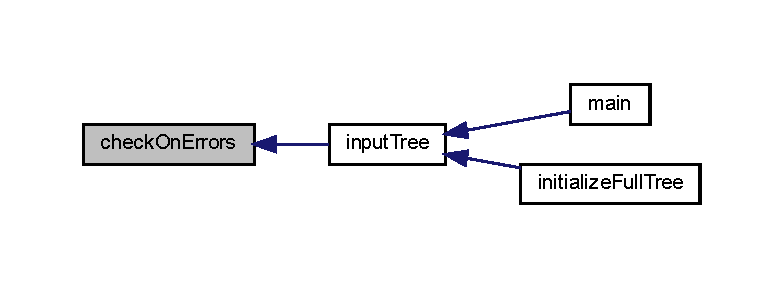
\includegraphics[width=350pt]{_open_brackets_8cpp_aaa006feb21d50122375e88727edfcfc7_icgraph}
\end{center}
\end{figure}
\mbox{\Hypertarget{_open_brackets_8cpp_ac803718224902c30b47da22d1d0e3cd6}\label{_open_brackets_8cpp_ac803718224902c30b47da22d1d0e3cd6}} 
\index{Open\+Brackets.\+cpp@{Open\+Brackets.\+cpp}!copy\+Vertex@{copy\+Vertex}}
\index{copy\+Vertex@{copy\+Vertex}!Open\+Brackets.\+cpp@{Open\+Brackets.\+cpp}}
\subsubsection{\texorpdfstring{copy\+Vertex()}{copyVertex()}}
{\footnotesize\ttfamily int copy\+Vertex (\begin{DoxyParamCaption}\item[{vector$<$ \mbox{\hyperlink{struct_node}{Node}} $>$ \&}]{tree,  }\item[{int}]{current\+Node }\end{DoxyParamCaption})}



Скопировать заданную вершину в векторе вершин 


\begin{DoxyParams}[1]{Аргументы}
\mbox{\tt in}  & {\em current\+Node} & индекс копируемой вершины \\
\hline
\mbox{\tt out}  & {\em tree} & вектор вершин \\
\hline
\end{DoxyParams}
\begin{DoxyReturn}{Возвращает}
индекс позиции скопированной вершины 
\end{DoxyReturn}
Граф вызовов\+:\nopagebreak
\begin{figure}[H]
\begin{center}
\leavevmode
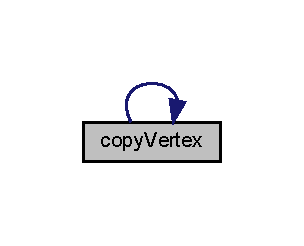
\includegraphics[width=146pt]{_open_brackets_8cpp_ac803718224902c30b47da22d1d0e3cd6_cgraph}
\end{center}
\end{figure}
Граф вызова функции\+:\nopagebreak
\begin{figure}[H]
\begin{center}
\leavevmode
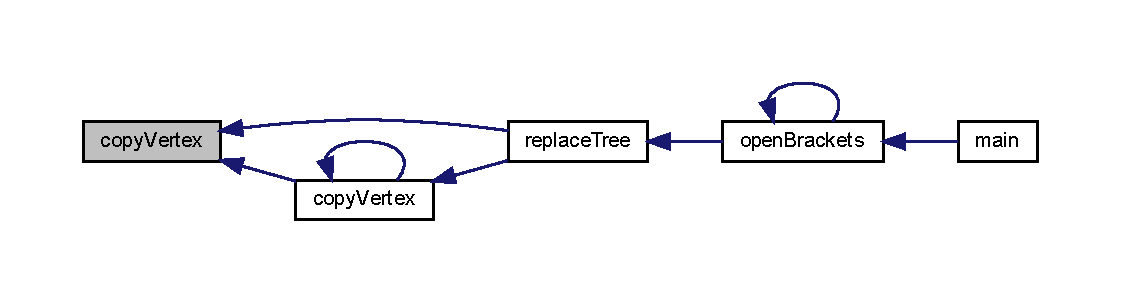
\includegraphics[width=350pt]{_open_brackets_8cpp_ac803718224902c30b47da22d1d0e3cd6_icgraph}
\end{center}
\end{figure}
\mbox{\Hypertarget{_open_brackets_8cpp_a0883c51a71859d6cb3eb32602e260e4c}\label{_open_brackets_8cpp_a0883c51a71859d6cb3eb32602e260e4c}} 
\index{Open\+Brackets.\+cpp@{Open\+Brackets.\+cpp}!crash\+Output@{crash\+Output}}
\index{crash\+Output@{crash\+Output}!Open\+Brackets.\+cpp@{Open\+Brackets.\+cpp}}
\subsubsection{\texorpdfstring{crash\+Output()}{crashOutput()}}
{\footnotesize\ttfamily bool crash\+Output (\begin{DoxyParamCaption}\item[{\mbox{\hyperlink{_open_brackets_header_8h_ab0df38968e4f03a3f1f6d6df0f31f45a}{Error\+Type}}}]{error }\end{DoxyParamCaption})}



Вывести сообщение об ошибке 


\begin{DoxyParams}[1]{Аргументы}
\mbox{\tt in}  & {\em error} & -\/ тип ошибки \\
\hline
\end{DoxyParams}
\begin{DoxyReturn}{Возвращает}
true при успешном выводе, false -\/ иначе 
\end{DoxyReturn}
Граф вызова функции\+:\nopagebreak
\begin{figure}[H]
\begin{center}
\leavevmode
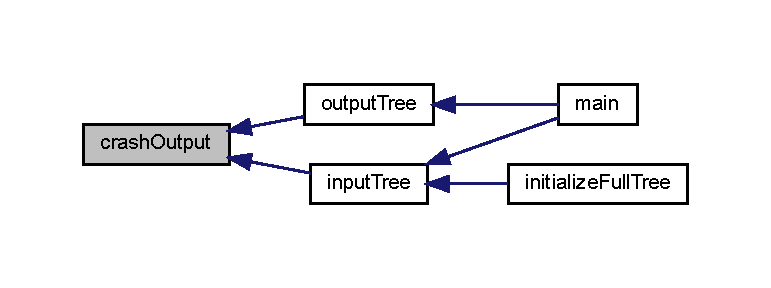
\includegraphics[width=350pt]{_open_brackets_8cpp_a0883c51a71859d6cb3eb32602e260e4c_icgraph}
\end{center}
\end{figure}
\mbox{\Hypertarget{_open_brackets_8cpp_ab583cc72190d7b0bc131d182dc947046}\label{_open_brackets_8cpp_ab583cc72190d7b0bc131d182dc947046}} 
\index{Open\+Brackets.\+cpp@{Open\+Brackets.\+cpp}!dfs\+Output@{dfs\+Output}}
\index{dfs\+Output@{dfs\+Output}!Open\+Brackets.\+cpp@{Open\+Brackets.\+cpp}}
\subsubsection{\texorpdfstring{dfs\+Output()}{dfsOutput()}}
{\footnotesize\ttfamily void dfs\+Output (\begin{DoxyParamCaption}\item[{ofstream \&}]{fout,  }\item[{vector$<$ \mbox{\hyperlink{struct_node}{Node}} $>$ \&}]{tree,  }\item[{int}]{current }\end{DoxyParamCaption})}



Вывести вершины дерева обходом в глубину 


\begin{DoxyParams}[1]{Аргументы}
\mbox{\tt in}  & {\em tree} & -\/ дерево разбора выражений \\
\hline
\mbox{\tt in}  & {\em current} & -\/ идентификатор вершины с которой производить вывод \\
\hline
\mbox{\tt out}  & {\em fout} & -\/ выходной поток \\
\hline
\end{DoxyParams}
Граф вызовов\+:\nopagebreak
\begin{figure}[H]
\begin{center}
\leavevmode
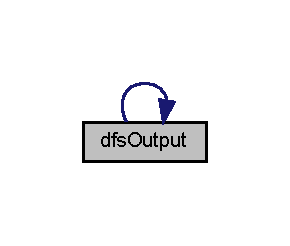
\includegraphics[width=139pt]{_open_brackets_8cpp_ab583cc72190d7b0bc131d182dc947046_cgraph}
\end{center}
\end{figure}
Граф вызова функции\+:\nopagebreak
\begin{figure}[H]
\begin{center}
\leavevmode
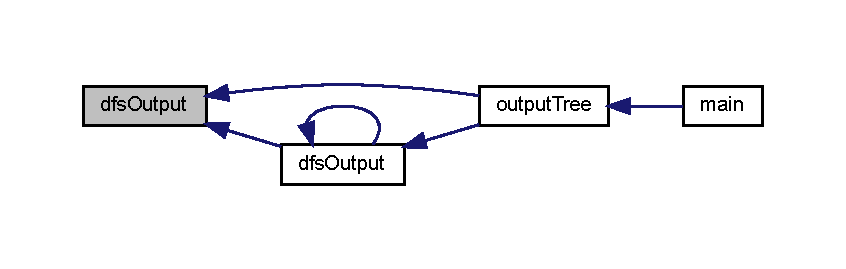
\includegraphics[width=350pt]{_open_brackets_8cpp_ab583cc72190d7b0bc131d182dc947046_icgraph}
\end{center}
\end{figure}
\mbox{\Hypertarget{_open_brackets_8cpp_a8e16eb9ea25217a287d10721c6d63e49}\label{_open_brackets_8cpp_a8e16eb9ea25217a287d10721c6d63e49}} 
\index{Open\+Brackets.\+cpp@{Open\+Brackets.\+cpp}!initialize\+Full\+Tree@{initialize\+Full\+Tree}}
\index{initialize\+Full\+Tree@{initialize\+Full\+Tree}!Open\+Brackets.\+cpp@{Open\+Brackets.\+cpp}}
\subsubsection{\texorpdfstring{initialize\+Full\+Tree()}{initializeFullTree()}}
{\footnotesize\ttfamily void initialize\+Full\+Tree (\begin{DoxyParamCaption}\item[{vector$<$ \mbox{\hyperlink{struct_node}{Node}} $>$ \&}]{input\+Tree }\end{DoxyParamCaption})}



Заполнить входное дерево до максимального размера 


\begin{DoxyParams}[1]{Аргументы}
\mbox{\tt out}  & {\em input\+Tree} & -\/ дерево разбора выражений \\
\hline
\end{DoxyParams}
Граф вызовов\+:\nopagebreak
\begin{figure}[H]
\begin{center}
\leavevmode
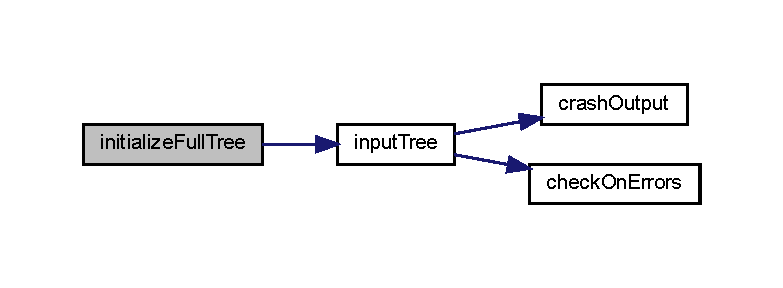
\includegraphics[width=350pt]{_open_brackets_8cpp_a8e16eb9ea25217a287d10721c6d63e49_cgraph}
\end{center}
\end{figure}
\mbox{\Hypertarget{_open_brackets_8cpp_a797b21a870af459209e0b303375490e6}\label{_open_brackets_8cpp_a797b21a870af459209e0b303375490e6}} 
\index{Open\+Brackets.\+cpp@{Open\+Brackets.\+cpp}!input\+Tree@{input\+Tree}}
\index{input\+Tree@{input\+Tree}!Open\+Brackets.\+cpp@{Open\+Brackets.\+cpp}}
\subsubsection{\texorpdfstring{input\+Tree()}{inputTree()}}
{\footnotesize\ttfamily bool input\+Tree (\begin{DoxyParamCaption}\item[{int}]{argc,  }\item[{char $\ast$}]{argv\mbox{[}$\,$\mbox{]},  }\item[{ifstream \&}]{fin,  }\item[{vector$<$ \mbox{\hyperlink{struct_node}{Node}} $>$ \&}]{tree,  }\item[{int \&}]{root }\end{DoxyParamCaption})}



Ввести заданное дерево разбора выражений 


\begin{DoxyParams}[1]{Аргументы}
\mbox{\tt in}  & {\em argc} & -\/ аргумент командной строки \\
\hline
\mbox{\tt in}  & {\em argv\mbox{[}$\,$\mbox{]}} & -\/ аргументы командной строки \\
\hline
\mbox{\tt in}  & {\em fin} & -\/ входной поток \\
\hline
\mbox{\tt out}  & {\em tree} & -\/ дерево разбора выражений \\
\hline
\mbox{\tt out}  & {\em root} & -\/ индекс корня дерева разбора выражений \\
\hline
\end{DoxyParams}
\begin{DoxyReturn}{Возвращает}
true -\/ при успешном ввводе, false -\/ иначе 
\end{DoxyReturn}

\begin{DoxyExceptions}{Исключения}
{\em U\+N\+K\+N\+O\+W\+N\+\_\+\+F\+I\+L\+E\+\_\+\+E\+X\+T\+E\+N\+S\+I\+ON} & -\/ неверно указано расширение входного файла \\
\hline
{\em I\+N\+P\+U\+T\+\_\+\+F\+I\+L\+E\+\_\+\+N\+O\+T\+\_\+\+E\+X\+I\+ST} & -\/ не существует или не найден входной файл \\
\hline
{\em W\+R\+O\+N\+G\+\_\+\+D\+A\+T\+A\+\_\+\+F\+O\+R\+M\+AT} & -\/ неверный формат данных во входном файле \\
\hline
{\em T\+R\+E\+E\+\_\+\+S\+I\+Z\+E\+\_\+\+O\+U\+T\+\_\+\+O\+F\+\_\+\+R\+A\+N\+GE} & -\/ размер дерева во входном файле вне поддерживаемого диапазона \\
\hline
\end{DoxyExceptions}
Граф вызовов\+:\nopagebreak
\begin{figure}[H]
\begin{center}
\leavevmode
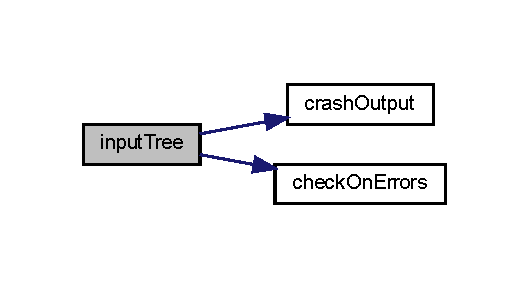
\includegraphics[width=254pt]{_open_brackets_8cpp_a797b21a870af459209e0b303375490e6_cgraph}
\end{center}
\end{figure}
Граф вызова функции\+:\nopagebreak
\begin{figure}[H]
\begin{center}
\leavevmode
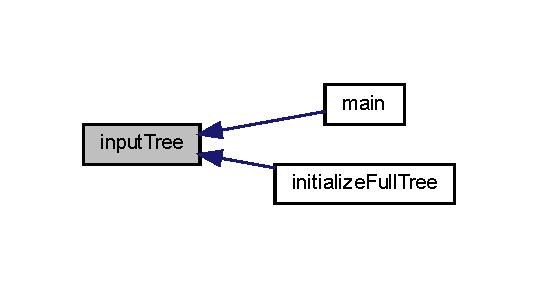
\includegraphics[width=258pt]{_open_brackets_8cpp_a797b21a870af459209e0b303375490e6_icgraph}
\end{center}
\end{figure}
\mbox{\Hypertarget{_open_brackets_8cpp_a25881c5367e2db6534a50cd6b17ed6a1}\label{_open_brackets_8cpp_a25881c5367e2db6534a50cd6b17ed6a1}} 
\index{Open\+Brackets.\+cpp@{Open\+Brackets.\+cpp}!is\+Equal\+Trees@{is\+Equal\+Trees}}
\index{is\+Equal\+Trees@{is\+Equal\+Trees}!Open\+Brackets.\+cpp@{Open\+Brackets.\+cpp}}
\subsubsection{\texorpdfstring{is\+Equal\+Trees()}{isEqualTrees()}}
{\footnotesize\ttfamily bool is\+Equal\+Trees (\begin{DoxyParamCaption}\item[{vector$<$ \mbox{\hyperlink{struct_node}{Node}} $>$}]{first\+Tree,  }\item[{int}]{root\+Of\+First\+Tree,  }\item[{vector$<$ \mbox{\hyperlink{struct_node}{Node}} $>$}]{second\+Tree,  }\item[{int}]{root\+Of\+Second\+Tree }\end{DoxyParamCaption})}



Сравнить два дерева между собой 


\begin{DoxyParams}[1]{Аргументы}
\mbox{\tt in}  & {\em first\+Tree} & -\/ первое дерево \\
\hline
\mbox{\tt in}  & {\em root\+Of\+First\+Tree} & -\/ индекс корневого узла первого дерева \\
\hline
\mbox{\tt in}  & {\em second\+Tree} & -\/ второе дерево \\
\hline
\mbox{\tt in}  & {\em root\+Of\+Second\+Tree} & -\/ индекс корневого узла второго дерева \\
\hline
\end{DoxyParams}
\begin{DoxyReturn}{Возвращает}
true -\/ если деревья совпадают, false -\/ если деревья разные 
\end{DoxyReturn}
Граф вызовов\+:\nopagebreak
\begin{figure}[H]
\begin{center}
\leavevmode
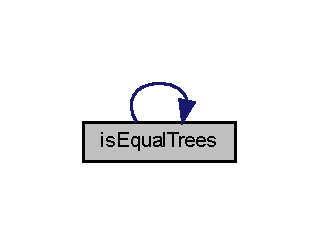
\includegraphics[width=153pt]{_open_brackets_8cpp_a25881c5367e2db6534a50cd6b17ed6a1_cgraph}
\end{center}
\end{figure}
Граф вызова функции\+:\nopagebreak
\begin{figure}[H]
\begin{center}
\leavevmode
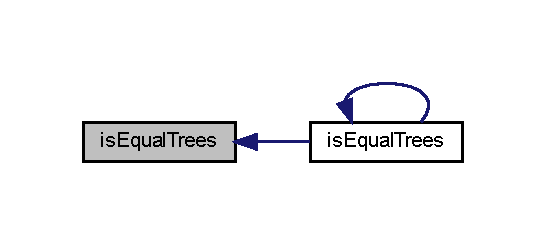
\includegraphics[width=262pt]{_open_brackets_8cpp_a25881c5367e2db6534a50cd6b17ed6a1_icgraph}
\end{center}
\end{figure}
\mbox{\Hypertarget{_open_brackets_8cpp_a0ddf1224851353fc92bfbff6f499fa97}\label{_open_brackets_8cpp_a0ddf1224851353fc92bfbff6f499fa97}} 
\index{Open\+Brackets.\+cpp@{Open\+Brackets.\+cpp}!main@{main}}
\index{main@{main}!Open\+Brackets.\+cpp@{Open\+Brackets.\+cpp}}
\subsubsection{\texorpdfstring{main()}{main()}}
{\footnotesize\ttfamily int main (\begin{DoxyParamCaption}\item[{int}]{argc,  }\item[{char $\ast$}]{argv\mbox{[}$\,$\mbox{]} }\end{DoxyParamCaption})}

Граф вызовов\+:\nopagebreak
\begin{figure}[H]
\begin{center}
\leavevmode
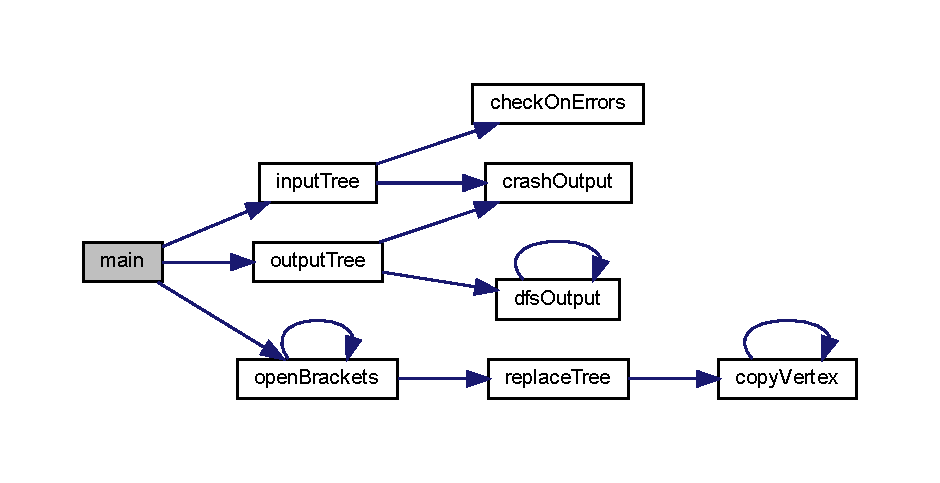
\includegraphics[width=350pt]{_open_brackets_8cpp_a0ddf1224851353fc92bfbff6f499fa97_cgraph}
\end{center}
\end{figure}
\mbox{\Hypertarget{_open_brackets_8cpp_a18dcaf2e91cb700bc12aae6fd594f0e8}\label{_open_brackets_8cpp_a18dcaf2e91cb700bc12aae6fd594f0e8}} 
\index{Open\+Brackets.\+cpp@{Open\+Brackets.\+cpp}!open\+Brackets@{open\+Brackets}}
\index{open\+Brackets@{open\+Brackets}!Open\+Brackets.\+cpp@{Open\+Brackets.\+cpp}}
\subsubsection{\texorpdfstring{open\+Brackets()}{openBrackets()}}
{\footnotesize\ttfamily void open\+Brackets (\begin{DoxyParamCaption}\item[{vector$<$ \mbox{\hyperlink{struct_node}{Node}} $>$ \&}]{tree,  }\item[{int}]{current\+Node }\end{DoxyParamCaption})}



Раскрыть скобки в заданном выражении 


\begin{DoxyParams}[1]{Аргументы}
\mbox{\tt in}  & {\em current\+Node} & -\/ индекс узла дерева с которого следует раскрывать скобки \\
\hline
\mbox{\tt out}  & {\em tree} & -\/ дерево разбора выражений \\
\hline
\end{DoxyParams}
Граф вызовов\+:\nopagebreak
\begin{figure}[H]
\begin{center}
\leavevmode
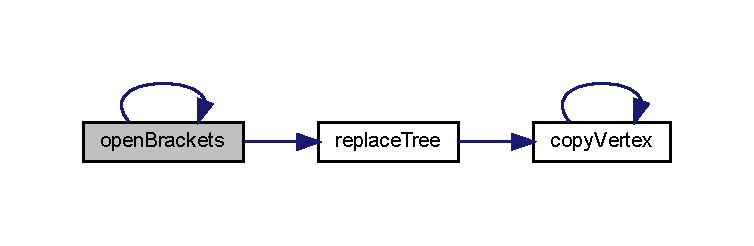
\includegraphics[width=350pt]{_open_brackets_8cpp_a18dcaf2e91cb700bc12aae6fd594f0e8_cgraph}
\end{center}
\end{figure}
Граф вызова функции\+:\nopagebreak
\begin{figure}[H]
\begin{center}
\leavevmode
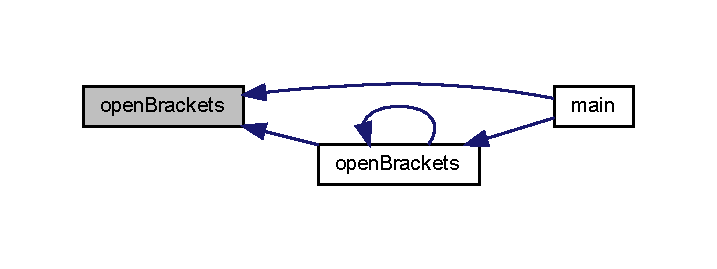
\includegraphics[width=344pt]{_open_brackets_8cpp_a18dcaf2e91cb700bc12aae6fd594f0e8_icgraph}
\end{center}
\end{figure}
\mbox{\Hypertarget{_open_brackets_8cpp_a7eb4dce1633fdd03c97d7fd46f02089f}\label{_open_brackets_8cpp_a7eb4dce1633fdd03c97d7fd46f02089f}} 
\index{Open\+Brackets.\+cpp@{Open\+Brackets.\+cpp}!output\+Tree@{output\+Tree}}
\index{output\+Tree@{output\+Tree}!Open\+Brackets.\+cpp@{Open\+Brackets.\+cpp}}
\subsubsection{\texorpdfstring{output\+Tree()}{outputTree()}}
{\footnotesize\ttfamily bool output\+Tree (\begin{DoxyParamCaption}\item[{int}]{argc,  }\item[{char $\ast$}]{argv\mbox{[}$\,$\mbox{]},  }\item[{ofstream \&}]{fout,  }\item[{vector$<$ \mbox{\hyperlink{struct_node}{Node}} $>$ \&}]{tree,  }\item[{int \&}]{current }\end{DoxyParamCaption})}



Вывести дерево разбора выражений 


\begin{DoxyParams}[1]{Аргументы}
\mbox{\tt in}  & {\em argc} & -\/ аргумент командной строки \\
\hline
\mbox{\tt in}  & {\em argv\mbox{[}$\,$\mbox{]}} & -\/ аргументы командной строки \\
\hline
\mbox{\tt in}  & {\em tree} & -\/ дерево разбора выражений \\
\hline
\mbox{\tt in}  & {\em current} & -\/ индекс вершины, с которой производить вывод дерева \\
\hline
\mbox{\tt out}  & {\em fout} & -\/ выходной поток \\
\hline
\end{DoxyParams}
\begin{DoxyReturn}{Возвращает}
true -\/ при успешном выводе, false -\/ иначе 
\end{DoxyReturn}

\begin{DoxyExceptions}{Исключения}
{\em U\+N\+K\+N\+O\+W\+N\+\_\+\+F\+I\+L\+E\+\_\+\+E\+X\+T\+E\+N\+S\+I\+ON} & -\/ неверно указано расширение выходного файла \\
\hline
{\em O\+U\+T\+P\+U\+T\+\_\+\+F\+I\+L\+E\+\_\+\+C\+R\+E\+A\+T\+I\+O\+N\+\_\+\+F\+A\+I\+L\+ED} & -\/ невозможно создать выходной файл \\
\hline
\end{DoxyExceptions}
Граф вызовов\+:\nopagebreak
\begin{figure}[H]
\begin{center}
\leavevmode
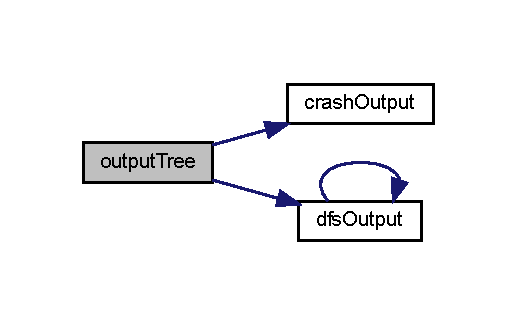
\includegraphics[width=248pt]{_open_brackets_8cpp_a7eb4dce1633fdd03c97d7fd46f02089f_cgraph}
\end{center}
\end{figure}
Граф вызова функции\+:\nopagebreak
\begin{figure}[H]
\begin{center}
\leavevmode
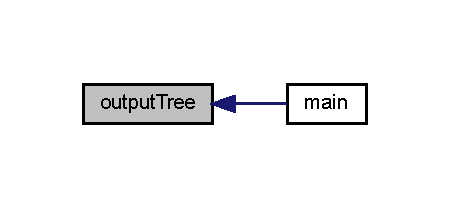
\includegraphics[width=216pt]{_open_brackets_8cpp_a7eb4dce1633fdd03c97d7fd46f02089f_icgraph}
\end{center}
\end{figure}
\mbox{\Hypertarget{_open_brackets_8cpp_a61492c3970be2433213dcd7344c27426}\label{_open_brackets_8cpp_a61492c3970be2433213dcd7344c27426}} 
\index{Open\+Brackets.\+cpp@{Open\+Brackets.\+cpp}!replace\+Tree@{replace\+Tree}}
\index{replace\+Tree@{replace\+Tree}!Open\+Brackets.\+cpp@{Open\+Brackets.\+cpp}}
\subsubsection{\texorpdfstring{replace\+Tree()}{replaceTree()}}
{\footnotesize\ttfamily void replace\+Tree (\begin{DoxyParamCaption}\item[{vector$<$ \mbox{\hyperlink{struct_node}{Node}} $>$ \&}]{tree,  }\item[{int}]{current\+Node,  }\item[{string}]{operation }\end{DoxyParamCaption})}



Перестроить часть дерева ниже текущего узла в соответствии с операцией 


\begin{DoxyParams}[1]{Аргументы}
\mbox{\tt in}  & {\em current\+Node} & -\/ индекс узла дерева с которого следует перестраивать дерево \\
\hline
\mbox{\tt in}  & {\em operation} & -\/ операция текущего узла \\
\hline
\mbox{\tt out}  & {\em tree} & -\/ дерево разбора выражений \\
\hline
\end{DoxyParams}
Граф вызовов\+:\nopagebreak
\begin{figure}[H]
\begin{center}
\leavevmode
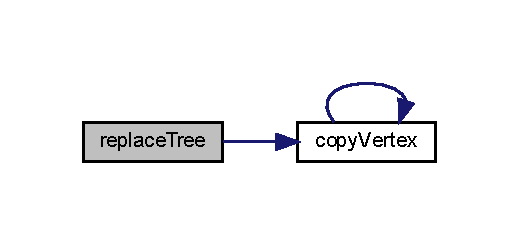
\includegraphics[width=249pt]{_open_brackets_8cpp_a61492c3970be2433213dcd7344c27426_cgraph}
\end{center}
\end{figure}
Граф вызова функции\+:\nopagebreak
\begin{figure}[H]
\begin{center}
\leavevmode
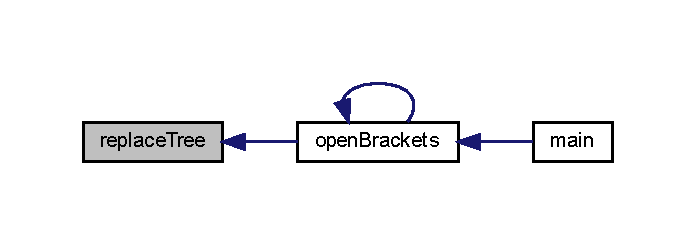
\includegraphics[width=334pt]{_open_brackets_8cpp_a61492c3970be2433213dcd7344c27426_icgraph}
\end{center}
\end{figure}

\hypertarget{_open_brackets_header_8h}{}\section{Файл Open\+Brackets\+Header.\+h}
\label{_open_brackets_header_8h}\index{Open\+Brackets\+Header.\+h@{Open\+Brackets\+Header.\+h}}


Заголовочный файл программы  


{\ttfamily \#include $<$vector$>$}\newline
\subsection*{Классы}
\begin{DoxyCompactItemize}
\item 
struct \mbox{\hyperlink{struct_node}{Node}}
\begin{DoxyCompactList}\small\item\em Узел дерева \end{DoxyCompactList}\end{DoxyCompactItemize}
\subsection*{Макросы}
\begin{DoxyCompactItemize}
\item 
\#define \mbox{\hyperlink{_open_brackets_header_8h_a85633b531a313eee6f1f31eeed4a12ea}{Max\+Size}}~30
\begin{DoxyCompactList}\small\item\em Максимальное число узлов в заданном дереве \end{DoxyCompactList}\item 
\#define \mbox{\hyperlink{_open_brackets_header_8h_a7802bc40fc347fd3fa6ff9ffc649429b}{Not\+Exist}}~-\/1
\begin{DoxyCompactList}\small\item\em Отсутствие узла \end{DoxyCompactList}\item 
\#define \mbox{\hyperlink{_open_brackets_header_8h_af08ec37a8c99d747fb60fa15bc28678b}{\+\_\+\+C\+R\+T\+\_\+\+S\+E\+C\+U\+R\+E\+\_\+\+N\+O\+\_\+\+W\+A\+R\+N\+I\+N\+GS}}
\begin{DoxyCompactList}\small\item\em Разрешить работу устаревшим функциям \end{DoxyCompactList}\end{DoxyCompactItemize}
\subsection*{Перечисления}
\begin{DoxyCompactItemize}
\item 
enum \mbox{\hyperlink{_open_brackets_header_8h_ab0df38968e4f03a3f1f6d6df0f31f45a}{Error\+Type}} \{ \newline
\mbox{\hyperlink{_open_brackets_header_8h_ab0df38968e4f03a3f1f6d6df0f31f45aabf350750d0d4fabd8954c0f1e9bbae94}{N\+O\+\_\+\+E\+R\+R\+OR}}, 
\mbox{\hyperlink{_open_brackets_header_8h_ab0df38968e4f03a3f1f6d6df0f31f45aa745c6dc5513b64293b0f7a07330eca5a}{I\+N\+P\+U\+T\+\_\+\+F\+I\+L\+E\+\_\+\+N\+O\+T\+\_\+\+E\+X\+I\+ST}}, 
\mbox{\hyperlink{_open_brackets_header_8h_ab0df38968e4f03a3f1f6d6df0f31f45aaff8a7487998c3d719774cffc052337eb}{U\+N\+K\+N\+O\+W\+N\+\_\+\+F\+I\+L\+E\+\_\+\+E\+X\+T\+E\+N\+S\+I\+ON}}, 
\mbox{\hyperlink{_open_brackets_header_8h_ab0df38968e4f03a3f1f6d6df0f31f45aa721018ff7b16779f8f5cafb4321277f8}{O\+U\+T\+P\+U\+T\+\_\+\+F\+I\+L\+E\+\_\+\+C\+R\+E\+A\+T\+I\+O\+N\+\_\+\+F\+A\+I\+L\+ED}}, 
\newline
\mbox{\hyperlink{_open_brackets_header_8h_ab0df38968e4f03a3f1f6d6df0f31f45aa476fbddd1a938cf0e1d5fbf07ce6b87e}{W\+R\+O\+N\+G\+\_\+\+D\+A\+T\+A\+\_\+\+F\+O\+R\+M\+AT}}, 
\mbox{\hyperlink{_open_brackets_header_8h_ab0df38968e4f03a3f1f6d6df0f31f45aaf3489c9ab89090205a7a28efc0b6d1c1}{N\+O\+T\+\_\+\+B\+I\+N\+A\+R\+Y\+\_\+\+T\+R\+EE}}, 
\mbox{\hyperlink{_open_brackets_header_8h_ab0df38968e4f03a3f1f6d6df0f31f45aa11e2c93ba3ff0e0954f481cff8c9e2e9}{S\+A\+M\+E\+\_\+\+N\+O\+D\+E\+S\+\_\+\+ID}}, 
\mbox{\hyperlink{_open_brackets_header_8h_ab0df38968e4f03a3f1f6d6df0f31f45aad20457f60c4a58cf7fa5d1cbd5acb402}{S\+A\+M\+E\+\_\+\+P\+A\+R\+E\+N\+T\+\_\+\+A\+N\+D\+\_\+\+N\+O\+D\+E\+\_\+\+ID}}, 
\newline
\mbox{\hyperlink{_open_brackets_header_8h_ab0df38968e4f03a3f1f6d6df0f31f45aa231effb1b46dd7f2fbb0b92f8253930a}{L\+A\+C\+K\+\_\+\+O\+F\+\_\+\+O\+P\+E\+R\+A\+N\+DS}}, 
\mbox{\hyperlink{_open_brackets_header_8h_ab0df38968e4f03a3f1f6d6df0f31f45aa7a4b0573feb2e22745595dfccabd98b7}{N\+O\+D\+E\+\_\+\+I\+D\+\_\+\+O\+U\+T\+\_\+\+O\+F\+\_\+\+R\+A\+N\+GE}}, 
\mbox{\hyperlink{_open_brackets_header_8h_ab0df38968e4f03a3f1f6d6df0f31f45aa51879bf6d8afa9b6c20983f5fa6ccb0d}{P\+A\+R\+E\+N\+T\+\_\+\+I\+D\+\_\+\+O\+U\+T\+\_\+\+O\+F\+\_\+\+R\+A\+N\+GE}}, 
\mbox{\hyperlink{_open_brackets_header_8h_ab0df38968e4f03a3f1f6d6df0f31f45aacc98ed2e6545b8f4b31b40fe065cca5e}{I\+N\+V\+A\+L\+I\+D\+\_\+\+N\+O\+D\+E\+\_\+\+S\+Y\+M\+B\+OL}}, 
\newline
\mbox{\hyperlink{_open_brackets_header_8h_ab0df38968e4f03a3f1f6d6df0f31f45aaf8be53c692c11fd616a06c54b9bc7931}{N\+O\+T\+\_\+\+R\+I\+G\+H\+T\+\_\+\+L\+I\+NK}}, 
\mbox{\hyperlink{_open_brackets_header_8h_ab0df38968e4f03a3f1f6d6df0f31f45aaaff55d7c59909f46ab5412cceed25f91}{U\+N\+E\+X\+C\+E\+P\+T\+A\+B\+L\+E\+\_\+\+P\+A\+R\+E\+N\+T\+\_\+\+ID}}, 
\mbox{\hyperlink{_open_brackets_header_8h_ab0df38968e4f03a3f1f6d6df0f31f45aa4511f7884272586e1906ce1ac45d4907}{N\+O\+\_\+\+R\+O\+OT}}, 
\mbox{\hyperlink{_open_brackets_header_8h_ab0df38968e4f03a3f1f6d6df0f31f45aad05d3d7ae27b3d7e4ce1cc2b805e32fa}{T\+R\+E\+E\+\_\+\+S\+I\+Z\+E\+\_\+\+O\+U\+T\+\_\+\+O\+F\+\_\+\+R\+A\+N\+GE}}, 
\newline
\mbox{\hyperlink{_open_brackets_header_8h_ab0df38968e4f03a3f1f6d6df0f31f45aa285b2afe35461f7a652a0761105c29a9}{I\+N\+V\+A\+L\+I\+D\+\_\+\+N\+U\+M\+B\+E\+R\+\_\+\+O\+F\+\_\+\+N\+O\+D\+ES}}
 \}
\begin{DoxyCompactList}\small\item\em Типы ошибок \end{DoxyCompactList}\end{DoxyCompactItemize}
\subsection*{Функции}
\begin{DoxyCompactItemize}
\item 
void \mbox{\hyperlink{_open_brackets_header_8h_a18dcaf2e91cb700bc12aae6fd594f0e8}{open\+Brackets}} (vector$<$ \mbox{\hyperlink{struct_node}{Node}} $>$ \&tree, int current\+Node)
\begin{DoxyCompactList}\small\item\em Раскрыть скобки в заданном выражении \end{DoxyCompactList}\item 
void \mbox{\hyperlink{_open_brackets_header_8h_a61492c3970be2433213dcd7344c27426}{replace\+Tree}} (vector$<$ \mbox{\hyperlink{struct_node}{Node}} $>$ \&tree, int current\+Node, string operation)
\begin{DoxyCompactList}\small\item\em Перестроить часть дерева ниже текущего узла в соответствии с операцией \end{DoxyCompactList}\item 
bool \mbox{\hyperlink{_open_brackets_header_8h_a0883c51a71859d6cb3eb32602e260e4c}{crash\+Output}} (\mbox{\hyperlink{_open_brackets_header_8h_ab0df38968e4f03a3f1f6d6df0f31f45a}{Error\+Type}} error)
\begin{DoxyCompactList}\small\item\em Вывести сообщение об ошибке \end{DoxyCompactList}\item 
\mbox{\hyperlink{_open_brackets_header_8h_ab0df38968e4f03a3f1f6d6df0f31f45a}{Error\+Type}} \mbox{\hyperlink{_open_brackets_header_8h_aaa006feb21d50122375e88727edfcfc7}{check\+On\+Errors}} (int \&size, vector$<$ \mbox{\hyperlink{struct_node}{Node}} $>$ \&tree, int \&root)
\begin{DoxyCompactList}\small\item\em Проверить дерево на ошибки \end{DoxyCompactList}\item 
bool \mbox{\hyperlink{_open_brackets_header_8h_a25881c5367e2db6534a50cd6b17ed6a1}{is\+Equal\+Trees}} (vector$<$ \mbox{\hyperlink{struct_node}{Node}} $>$ first\+Tree, int root\+Of\+First\+Tree, vector$<$ \mbox{\hyperlink{struct_node}{Node}} $>$ second\+Tree, int root\+Of\+Second\+Tree)
\begin{DoxyCompactList}\small\item\em Сравнить два дерева между собой \end{DoxyCompactList}\item 
void \mbox{\hyperlink{_open_brackets_header_8h_a8e16eb9ea25217a287d10721c6d63e49}{initialize\+Full\+Tree}} (vector$<$ \mbox{\hyperlink{struct_node}{Node}} $>$ \&\mbox{\hyperlink{_open_brackets_header_8h_a797b21a870af459209e0b303375490e6}{input\+Tree}})
\begin{DoxyCompactList}\small\item\em Заполнить входное дерево до максимального размера \end{DoxyCompactList}\item 
bool \mbox{\hyperlink{_open_brackets_header_8h_a797b21a870af459209e0b303375490e6}{input\+Tree}} (int argc, char $\ast$argv\mbox{[}$\,$\mbox{]}, ifstream \&fin, vector$<$ \mbox{\hyperlink{struct_node}{Node}} $>$ \&tree, int \&root)
\begin{DoxyCompactList}\small\item\em Ввести заданное дерево разбора выражений \end{DoxyCompactList}\item 
bool \mbox{\hyperlink{_open_brackets_header_8h_a7eb4dce1633fdd03c97d7fd46f02089f}{output\+Tree}} (int argc, char $\ast$argv\mbox{[}$\,$\mbox{]}, ofstream \&fout, vector$<$ \mbox{\hyperlink{struct_node}{Node}} $>$ \&tree, int \&current)
\begin{DoxyCompactList}\small\item\em Вывести дерево разбора выражений \end{DoxyCompactList}\item 
void \mbox{\hyperlink{_open_brackets_header_8h_ab583cc72190d7b0bc131d182dc947046}{dfs\+Output}} (ofstream \&fout, vector$<$ \mbox{\hyperlink{struct_node}{Node}} $>$ \&tree, int current)
\begin{DoxyCompactList}\small\item\em Вывести вершины дерева обходом в глубину \end{DoxyCompactList}\item 
int \mbox{\hyperlink{_open_brackets_header_8h_ac803718224902c30b47da22d1d0e3cd6}{copy\+Vertex}} (vector$<$ \mbox{\hyperlink{struct_node}{Node}} $>$ \&tree, int current\+Node)
\begin{DoxyCompactList}\small\item\em Скопировать заданную вершину в векторе вершин \end{DoxyCompactList}\end{DoxyCompactItemize}


\subsection{Подробное описание}
Заголовочный файл программы 

Файл содержит в себе структуры и заголовки для функций программы, раскрываюшей скобки в математическом выражении, заданном деревом разбора выражений в виде списка смежности. 

\subsection{Макросы}
\mbox{\Hypertarget{_open_brackets_header_8h_af08ec37a8c99d747fb60fa15bc28678b}\label{_open_brackets_header_8h_af08ec37a8c99d747fb60fa15bc28678b}} 
\index{Open\+Brackets\+Header.\+h@{Open\+Brackets\+Header.\+h}!\+\_\+\+C\+R\+T\+\_\+\+S\+E\+C\+U\+R\+E\+\_\+\+N\+O\+\_\+\+W\+A\+R\+N\+I\+N\+GS@{\+\_\+\+C\+R\+T\+\_\+\+S\+E\+C\+U\+R\+E\+\_\+\+N\+O\+\_\+\+W\+A\+R\+N\+I\+N\+GS}}
\index{\+\_\+\+C\+R\+T\+\_\+\+S\+E\+C\+U\+R\+E\+\_\+\+N\+O\+\_\+\+W\+A\+R\+N\+I\+N\+GS@{\+\_\+\+C\+R\+T\+\_\+\+S\+E\+C\+U\+R\+E\+\_\+\+N\+O\+\_\+\+W\+A\+R\+N\+I\+N\+GS}!Open\+Brackets\+Header.\+h@{Open\+Brackets\+Header.\+h}}
\subsubsection{\texorpdfstring{\+\_\+\+C\+R\+T\+\_\+\+S\+E\+C\+U\+R\+E\+\_\+\+N\+O\+\_\+\+W\+A\+R\+N\+I\+N\+GS}{\_CRT\_SECURE\_NO\_WARNINGS}}
{\footnotesize\ttfamily \#define \+\_\+\+C\+R\+T\+\_\+\+S\+E\+C\+U\+R\+E\+\_\+\+N\+O\+\_\+\+W\+A\+R\+N\+I\+N\+GS}



Разрешить работу устаревшим функциям 

\mbox{\Hypertarget{_open_brackets_header_8h_a85633b531a313eee6f1f31eeed4a12ea}\label{_open_brackets_header_8h_a85633b531a313eee6f1f31eeed4a12ea}} 
\index{Open\+Brackets\+Header.\+h@{Open\+Brackets\+Header.\+h}!Max\+Size@{Max\+Size}}
\index{Max\+Size@{Max\+Size}!Open\+Brackets\+Header.\+h@{Open\+Brackets\+Header.\+h}}
\subsubsection{\texorpdfstring{Max\+Size}{MaxSize}}
{\footnotesize\ttfamily \#define Max\+Size~30}



Максимальное число узлов в заданном дереве 

\mbox{\Hypertarget{_open_brackets_header_8h_a7802bc40fc347fd3fa6ff9ffc649429b}\label{_open_brackets_header_8h_a7802bc40fc347fd3fa6ff9ffc649429b}} 
\index{Open\+Brackets\+Header.\+h@{Open\+Brackets\+Header.\+h}!Not\+Exist@{Not\+Exist}}
\index{Not\+Exist@{Not\+Exist}!Open\+Brackets\+Header.\+h@{Open\+Brackets\+Header.\+h}}
\subsubsection{\texorpdfstring{Not\+Exist}{NotExist}}
{\footnotesize\ttfamily \#define Not\+Exist~-\/1}



Отсутствие узла 



\subsection{Перечисления}
\mbox{\Hypertarget{_open_brackets_header_8h_ab0df38968e4f03a3f1f6d6df0f31f45a}\label{_open_brackets_header_8h_ab0df38968e4f03a3f1f6d6df0f31f45a}} 
\index{Open\+Brackets\+Header.\+h@{Open\+Brackets\+Header.\+h}!Error\+Type@{Error\+Type}}
\index{Error\+Type@{Error\+Type}!Open\+Brackets\+Header.\+h@{Open\+Brackets\+Header.\+h}}
\subsubsection{\texorpdfstring{Error\+Type}{ErrorType}}
{\footnotesize\ttfamily enum \mbox{\hyperlink{_open_brackets_header_8h_ab0df38968e4f03a3f1f6d6df0f31f45a}{Error\+Type}}}



Типы ошибок 

\begin{DoxyEnumFields}{Элементы перечислений}
\raisebox{\heightof{T}}[0pt][0pt]{\index{N\+O\+\_\+\+E\+R\+R\+OR@{N\+O\+\_\+\+E\+R\+R\+OR}!Open\+Brackets\+Header.\+h@{Open\+Brackets\+Header.\+h}}\index{Open\+Brackets\+Header.\+h@{Open\+Brackets\+Header.\+h}!N\+O\+\_\+\+E\+R\+R\+OR@{N\+O\+\_\+\+E\+R\+R\+OR}}}\mbox{\Hypertarget{_open_brackets_header_8h_ab0df38968e4f03a3f1f6d6df0f31f45aabf350750d0d4fabd8954c0f1e9bbae94}\label{_open_brackets_header_8h_ab0df38968e4f03a3f1f6d6df0f31f45aabf350750d0d4fabd8954c0f1e9bbae94}} 
N\+O\+\_\+\+E\+R\+R\+OR&Нет ошибки \\
\hline

\raisebox{\heightof{T}}[0pt][0pt]{\index{I\+N\+P\+U\+T\+\_\+\+F\+I\+L\+E\+\_\+\+N\+O\+T\+\_\+\+E\+X\+I\+ST@{I\+N\+P\+U\+T\+\_\+\+F\+I\+L\+E\+\_\+\+N\+O\+T\+\_\+\+E\+X\+I\+ST}!Open\+Brackets\+Header.\+h@{Open\+Brackets\+Header.\+h}}\index{Open\+Brackets\+Header.\+h@{Open\+Brackets\+Header.\+h}!I\+N\+P\+U\+T\+\_\+\+F\+I\+L\+E\+\_\+\+N\+O\+T\+\_\+\+E\+X\+I\+ST@{I\+N\+P\+U\+T\+\_\+\+F\+I\+L\+E\+\_\+\+N\+O\+T\+\_\+\+E\+X\+I\+ST}}}\mbox{\Hypertarget{_open_brackets_header_8h_ab0df38968e4f03a3f1f6d6df0f31f45aa745c6dc5513b64293b0f7a07330eca5a}\label{_open_brackets_header_8h_ab0df38968e4f03a3f1f6d6df0f31f45aa745c6dc5513b64293b0f7a07330eca5a}} 
I\+N\+P\+U\+T\+\_\+\+F\+I\+L\+E\+\_\+\+N\+O\+T\+\_\+\+E\+X\+I\+ST&Входной файл не существует \\
\hline

\raisebox{\heightof{T}}[0pt][0pt]{\index{U\+N\+K\+N\+O\+W\+N\+\_\+\+F\+I\+L\+E\+\_\+\+E\+X\+T\+E\+N\+S\+I\+ON@{U\+N\+K\+N\+O\+W\+N\+\_\+\+F\+I\+L\+E\+\_\+\+E\+X\+T\+E\+N\+S\+I\+ON}!Open\+Brackets\+Header.\+h@{Open\+Brackets\+Header.\+h}}\index{Open\+Brackets\+Header.\+h@{Open\+Brackets\+Header.\+h}!U\+N\+K\+N\+O\+W\+N\+\_\+\+F\+I\+L\+E\+\_\+\+E\+X\+T\+E\+N\+S\+I\+ON@{U\+N\+K\+N\+O\+W\+N\+\_\+\+F\+I\+L\+E\+\_\+\+E\+X\+T\+E\+N\+S\+I\+ON}}}\mbox{\Hypertarget{_open_brackets_header_8h_ab0df38968e4f03a3f1f6d6df0f31f45aaff8a7487998c3d719774cffc052337eb}\label{_open_brackets_header_8h_ab0df38968e4f03a3f1f6d6df0f31f45aaff8a7487998c3d719774cffc052337eb}} 
U\+N\+K\+N\+O\+W\+N\+\_\+\+F\+I\+L\+E\+\_\+\+E\+X\+T\+E\+N\+S\+I\+ON&Входной файл имеет неправильное расширение \\
\hline

\raisebox{\heightof{T}}[0pt][0pt]{\index{O\+U\+T\+P\+U\+T\+\_\+\+F\+I\+L\+E\+\_\+\+C\+R\+E\+A\+T\+I\+O\+N\+\_\+\+F\+A\+I\+L\+ED@{O\+U\+T\+P\+U\+T\+\_\+\+F\+I\+L\+E\+\_\+\+C\+R\+E\+A\+T\+I\+O\+N\+\_\+\+F\+A\+I\+L\+ED}!Open\+Brackets\+Header.\+h@{Open\+Brackets\+Header.\+h}}\index{Open\+Brackets\+Header.\+h@{Open\+Brackets\+Header.\+h}!O\+U\+T\+P\+U\+T\+\_\+\+F\+I\+L\+E\+\_\+\+C\+R\+E\+A\+T\+I\+O\+N\+\_\+\+F\+A\+I\+L\+ED@{O\+U\+T\+P\+U\+T\+\_\+\+F\+I\+L\+E\+\_\+\+C\+R\+E\+A\+T\+I\+O\+N\+\_\+\+F\+A\+I\+L\+ED}}}\mbox{\Hypertarget{_open_brackets_header_8h_ab0df38968e4f03a3f1f6d6df0f31f45aa721018ff7b16779f8f5cafb4321277f8}\label{_open_brackets_header_8h_ab0df38968e4f03a3f1f6d6df0f31f45aa721018ff7b16779f8f5cafb4321277f8}} 
O\+U\+T\+P\+U\+T\+\_\+\+F\+I\+L\+E\+\_\+\+C\+R\+E\+A\+T\+I\+O\+N\+\_\+\+F\+A\+I\+L\+ED&Невозможно создать указанный выходной файл \\
\hline

\raisebox{\heightof{T}}[0pt][0pt]{\index{W\+R\+O\+N\+G\+\_\+\+D\+A\+T\+A\+\_\+\+F\+O\+R\+M\+AT@{W\+R\+O\+N\+G\+\_\+\+D\+A\+T\+A\+\_\+\+F\+O\+R\+M\+AT}!Open\+Brackets\+Header.\+h@{Open\+Brackets\+Header.\+h}}\index{Open\+Brackets\+Header.\+h@{Open\+Brackets\+Header.\+h}!W\+R\+O\+N\+G\+\_\+\+D\+A\+T\+A\+\_\+\+F\+O\+R\+M\+AT@{W\+R\+O\+N\+G\+\_\+\+D\+A\+T\+A\+\_\+\+F\+O\+R\+M\+AT}}}\mbox{\Hypertarget{_open_brackets_header_8h_ab0df38968e4f03a3f1f6d6df0f31f45aa476fbddd1a938cf0e1d5fbf07ce6b87e}\label{_open_brackets_header_8h_ab0df38968e4f03a3f1f6d6df0f31f45aa476fbddd1a938cf0e1d5fbf07ce6b87e}} 
W\+R\+O\+N\+G\+\_\+\+D\+A\+T\+A\+\_\+\+F\+O\+R\+M\+AT&Во входном файле формат предоставляемых данных не соответствует требуемому \\
\hline

\raisebox{\heightof{T}}[0pt][0pt]{\index{N\+O\+T\+\_\+\+B\+I\+N\+A\+R\+Y\+\_\+\+T\+R\+EE@{N\+O\+T\+\_\+\+B\+I\+N\+A\+R\+Y\+\_\+\+T\+R\+EE}!Open\+Brackets\+Header.\+h@{Open\+Brackets\+Header.\+h}}\index{Open\+Brackets\+Header.\+h@{Open\+Brackets\+Header.\+h}!N\+O\+T\+\_\+\+B\+I\+N\+A\+R\+Y\+\_\+\+T\+R\+EE@{N\+O\+T\+\_\+\+B\+I\+N\+A\+R\+Y\+\_\+\+T\+R\+EE}}}\mbox{\Hypertarget{_open_brackets_header_8h_ab0df38968e4f03a3f1f6d6df0f31f45aaf3489c9ab89090205a7a28efc0b6d1c1}\label{_open_brackets_header_8h_ab0df38968e4f03a3f1f6d6df0f31f45aaf3489c9ab89090205a7a28efc0b6d1c1}} 
N\+O\+T\+\_\+\+B\+I\+N\+A\+R\+Y\+\_\+\+T\+R\+EE&У узлов дерева разбора выражений больше двух детей \\
\hline

\raisebox{\heightof{T}}[0pt][0pt]{\index{S\+A\+M\+E\+\_\+\+N\+O\+D\+E\+S\+\_\+\+ID@{S\+A\+M\+E\+\_\+\+N\+O\+D\+E\+S\+\_\+\+ID}!Open\+Brackets\+Header.\+h@{Open\+Brackets\+Header.\+h}}\index{Open\+Brackets\+Header.\+h@{Open\+Brackets\+Header.\+h}!S\+A\+M\+E\+\_\+\+N\+O\+D\+E\+S\+\_\+\+ID@{S\+A\+M\+E\+\_\+\+N\+O\+D\+E\+S\+\_\+\+ID}}}\mbox{\Hypertarget{_open_brackets_header_8h_ab0df38968e4f03a3f1f6d6df0f31f45aa11e2c93ba3ff0e0954f481cff8c9e2e9}\label{_open_brackets_header_8h_ab0df38968e4f03a3f1f6d6df0f31f45aa11e2c93ba3ff0e0954f481cff8c9e2e9}} 
S\+A\+M\+E\+\_\+\+N\+O\+D\+E\+S\+\_\+\+ID&Идентификаторы узлов совпадают \\
\hline

\raisebox{\heightof{T}}[0pt][0pt]{\index{S\+A\+M\+E\+\_\+\+P\+A\+R\+E\+N\+T\+\_\+\+A\+N\+D\+\_\+\+N\+O\+D\+E\+\_\+\+ID@{S\+A\+M\+E\+\_\+\+P\+A\+R\+E\+N\+T\+\_\+\+A\+N\+D\+\_\+\+N\+O\+D\+E\+\_\+\+ID}!Open\+Brackets\+Header.\+h@{Open\+Brackets\+Header.\+h}}\index{Open\+Brackets\+Header.\+h@{Open\+Brackets\+Header.\+h}!S\+A\+M\+E\+\_\+\+P\+A\+R\+E\+N\+T\+\_\+\+A\+N\+D\+\_\+\+N\+O\+D\+E\+\_\+\+ID@{S\+A\+M\+E\+\_\+\+P\+A\+R\+E\+N\+T\+\_\+\+A\+N\+D\+\_\+\+N\+O\+D\+E\+\_\+\+ID}}}\mbox{\Hypertarget{_open_brackets_header_8h_ab0df38968e4f03a3f1f6d6df0f31f45aad20457f60c4a58cf7fa5d1cbd5acb402}\label{_open_brackets_header_8h_ab0df38968e4f03a3f1f6d6df0f31f45aad20457f60c4a58cf7fa5d1cbd5acb402}} 
S\+A\+M\+E\+\_\+\+P\+A\+R\+E\+N\+T\+\_\+\+A\+N\+D\+\_\+\+N\+O\+D\+E\+\_\+\+ID&Идентификатор родительского узла совпадает с идентификатором узла \\
\hline

\raisebox{\heightof{T}}[0pt][0pt]{\index{L\+A\+C\+K\+\_\+\+O\+F\+\_\+\+O\+P\+E\+R\+A\+N\+DS@{L\+A\+C\+K\+\_\+\+O\+F\+\_\+\+O\+P\+E\+R\+A\+N\+DS}!Open\+Brackets\+Header.\+h@{Open\+Brackets\+Header.\+h}}\index{Open\+Brackets\+Header.\+h@{Open\+Brackets\+Header.\+h}!L\+A\+C\+K\+\_\+\+O\+F\+\_\+\+O\+P\+E\+R\+A\+N\+DS@{L\+A\+C\+K\+\_\+\+O\+F\+\_\+\+O\+P\+E\+R\+A\+N\+DS}}}\mbox{\Hypertarget{_open_brackets_header_8h_ab0df38968e4f03a3f1f6d6df0f31f45aa231effb1b46dd7f2fbb0b92f8253930a}\label{_open_brackets_header_8h_ab0df38968e4f03a3f1f6d6df0f31f45aa231effb1b46dd7f2fbb0b92f8253930a}} 
L\+A\+C\+K\+\_\+\+O\+F\+\_\+\+O\+P\+E\+R\+A\+N\+DS&У операции слишком мало операндов \\
\hline

\raisebox{\heightof{T}}[0pt][0pt]{\index{N\+O\+D\+E\+\_\+\+I\+D\+\_\+\+O\+U\+T\+\_\+\+O\+F\+\_\+\+R\+A\+N\+GE@{N\+O\+D\+E\+\_\+\+I\+D\+\_\+\+O\+U\+T\+\_\+\+O\+F\+\_\+\+R\+A\+N\+GE}!Open\+Brackets\+Header.\+h@{Open\+Brackets\+Header.\+h}}\index{Open\+Brackets\+Header.\+h@{Open\+Brackets\+Header.\+h}!N\+O\+D\+E\+\_\+\+I\+D\+\_\+\+O\+U\+T\+\_\+\+O\+F\+\_\+\+R\+A\+N\+GE@{N\+O\+D\+E\+\_\+\+I\+D\+\_\+\+O\+U\+T\+\_\+\+O\+F\+\_\+\+R\+A\+N\+GE}}}\mbox{\Hypertarget{_open_brackets_header_8h_ab0df38968e4f03a3f1f6d6df0f31f45aa7a4b0573feb2e22745595dfccabd98b7}\label{_open_brackets_header_8h_ab0df38968e4f03a3f1f6d6df0f31f45aa7a4b0573feb2e22745595dfccabd98b7}} 
N\+O\+D\+E\+\_\+\+I\+D\+\_\+\+O\+U\+T\+\_\+\+O\+F\+\_\+\+R\+A\+N\+GE&Идентификатор узла дерева разбора выражений вне поддерживаемого диапазона \\
\hline

\raisebox{\heightof{T}}[0pt][0pt]{\index{P\+A\+R\+E\+N\+T\+\_\+\+I\+D\+\_\+\+O\+U\+T\+\_\+\+O\+F\+\_\+\+R\+A\+N\+GE@{P\+A\+R\+E\+N\+T\+\_\+\+I\+D\+\_\+\+O\+U\+T\+\_\+\+O\+F\+\_\+\+R\+A\+N\+GE}!Open\+Brackets\+Header.\+h@{Open\+Brackets\+Header.\+h}}\index{Open\+Brackets\+Header.\+h@{Open\+Brackets\+Header.\+h}!P\+A\+R\+E\+N\+T\+\_\+\+I\+D\+\_\+\+O\+U\+T\+\_\+\+O\+F\+\_\+\+R\+A\+N\+GE@{P\+A\+R\+E\+N\+T\+\_\+\+I\+D\+\_\+\+O\+U\+T\+\_\+\+O\+F\+\_\+\+R\+A\+N\+GE}}}\mbox{\Hypertarget{_open_brackets_header_8h_ab0df38968e4f03a3f1f6d6df0f31f45aa51879bf6d8afa9b6c20983f5fa6ccb0d}\label{_open_brackets_header_8h_ab0df38968e4f03a3f1f6d6df0f31f45aa51879bf6d8afa9b6c20983f5fa6ccb0d}} 
P\+A\+R\+E\+N\+T\+\_\+\+I\+D\+\_\+\+O\+U\+T\+\_\+\+O\+F\+\_\+\+R\+A\+N\+GE&Идентификатор родительского узла для узла в дереве разбора выражений вне поддерживаемого диапазона \\
\hline

\raisebox{\heightof{T}}[0pt][0pt]{\index{I\+N\+V\+A\+L\+I\+D\+\_\+\+N\+O\+D\+E\+\_\+\+S\+Y\+M\+B\+OL@{I\+N\+V\+A\+L\+I\+D\+\_\+\+N\+O\+D\+E\+\_\+\+S\+Y\+M\+B\+OL}!Open\+Brackets\+Header.\+h@{Open\+Brackets\+Header.\+h}}\index{Open\+Brackets\+Header.\+h@{Open\+Brackets\+Header.\+h}!I\+N\+V\+A\+L\+I\+D\+\_\+\+N\+O\+D\+E\+\_\+\+S\+Y\+M\+B\+OL@{I\+N\+V\+A\+L\+I\+D\+\_\+\+N\+O\+D\+E\+\_\+\+S\+Y\+M\+B\+OL}}}\mbox{\Hypertarget{_open_brackets_header_8h_ab0df38968e4f03a3f1f6d6df0f31f45aacc98ed2e6545b8f4b31b40fe065cca5e}\label{_open_brackets_header_8h_ab0df38968e4f03a3f1f6d6df0f31f45aacc98ed2e6545b8f4b31b40fe065cca5e}} 
I\+N\+V\+A\+L\+I\+D\+\_\+\+N\+O\+D\+E\+\_\+\+S\+Y\+M\+B\+OL&Недопустимый символ в значении операнда \\
\hline

\raisebox{\heightof{T}}[0pt][0pt]{\index{N\+O\+T\+\_\+\+R\+I\+G\+H\+T\+\_\+\+L\+I\+NK@{N\+O\+T\+\_\+\+R\+I\+G\+H\+T\+\_\+\+L\+I\+NK}!Open\+Brackets\+Header.\+h@{Open\+Brackets\+Header.\+h}}\index{Open\+Brackets\+Header.\+h@{Open\+Brackets\+Header.\+h}!N\+O\+T\+\_\+\+R\+I\+G\+H\+T\+\_\+\+L\+I\+NK@{N\+O\+T\+\_\+\+R\+I\+G\+H\+T\+\_\+\+L\+I\+NK}}}\mbox{\Hypertarget{_open_brackets_header_8h_ab0df38968e4f03a3f1f6d6df0f31f45aaf8be53c692c11fd616a06c54b9bc7931}\label{_open_brackets_header_8h_ab0df38968e4f03a3f1f6d6df0f31f45aaf8be53c692c11fd616a06c54b9bc7931}} 
N\+O\+T\+\_\+\+R\+I\+G\+H\+T\+\_\+\+L\+I\+NK&Родители и дети у узлов не совпадают \\
\hline

\raisebox{\heightof{T}}[0pt][0pt]{\index{U\+N\+E\+X\+C\+E\+P\+T\+A\+B\+L\+E\+\_\+\+P\+A\+R\+E\+N\+T\+\_\+\+ID@{U\+N\+E\+X\+C\+E\+P\+T\+A\+B\+L\+E\+\_\+\+P\+A\+R\+E\+N\+T\+\_\+\+ID}!Open\+Brackets\+Header.\+h@{Open\+Brackets\+Header.\+h}}\index{Open\+Brackets\+Header.\+h@{Open\+Brackets\+Header.\+h}!U\+N\+E\+X\+C\+E\+P\+T\+A\+B\+L\+E\+\_\+\+P\+A\+R\+E\+N\+T\+\_\+\+ID@{U\+N\+E\+X\+C\+E\+P\+T\+A\+B\+L\+E\+\_\+\+P\+A\+R\+E\+N\+T\+\_\+\+ID}}}\mbox{\Hypertarget{_open_brackets_header_8h_ab0df38968e4f03a3f1f6d6df0f31f45aaaff55d7c59909f46ab5412cceed25f91}\label{_open_brackets_header_8h_ab0df38968e4f03a3f1f6d6df0f31f45aaaff55d7c59909f46ab5412cceed25f91}} 
U\+N\+E\+X\+C\+E\+P\+T\+A\+B\+L\+E\+\_\+\+P\+A\+R\+E\+N\+T\+\_\+\+ID&Идентификатор родительского узла является идентификатором узла-\/ребёнка \\
\hline

\raisebox{\heightof{T}}[0pt][0pt]{\index{N\+O\+\_\+\+R\+O\+OT@{N\+O\+\_\+\+R\+O\+OT}!Open\+Brackets\+Header.\+h@{Open\+Brackets\+Header.\+h}}\index{Open\+Brackets\+Header.\+h@{Open\+Brackets\+Header.\+h}!N\+O\+\_\+\+R\+O\+OT@{N\+O\+\_\+\+R\+O\+OT}}}\mbox{\Hypertarget{_open_brackets_header_8h_ab0df38968e4f03a3f1f6d6df0f31f45aa4511f7884272586e1906ce1ac45d4907}\label{_open_brackets_header_8h_ab0df38968e4f03a3f1f6d6df0f31f45aa4511f7884272586e1906ce1ac45d4907}} 
N\+O\+\_\+\+R\+O\+OT&Отсутствие корневого узла \\
\hline

\raisebox{\heightof{T}}[0pt][0pt]{\index{T\+R\+E\+E\+\_\+\+S\+I\+Z\+E\+\_\+\+O\+U\+T\+\_\+\+O\+F\+\_\+\+R\+A\+N\+GE@{T\+R\+E\+E\+\_\+\+S\+I\+Z\+E\+\_\+\+O\+U\+T\+\_\+\+O\+F\+\_\+\+R\+A\+N\+GE}!Open\+Brackets\+Header.\+h@{Open\+Brackets\+Header.\+h}}\index{Open\+Brackets\+Header.\+h@{Open\+Brackets\+Header.\+h}!T\+R\+E\+E\+\_\+\+S\+I\+Z\+E\+\_\+\+O\+U\+T\+\_\+\+O\+F\+\_\+\+R\+A\+N\+GE@{T\+R\+E\+E\+\_\+\+S\+I\+Z\+E\+\_\+\+O\+U\+T\+\_\+\+O\+F\+\_\+\+R\+A\+N\+GE}}}\mbox{\Hypertarget{_open_brackets_header_8h_ab0df38968e4f03a3f1f6d6df0f31f45aad05d3d7ae27b3d7e4ce1cc2b805e32fa}\label{_open_brackets_header_8h_ab0df38968e4f03a3f1f6d6df0f31f45aad05d3d7ae27b3d7e4ce1cc2b805e32fa}} 
T\+R\+E\+E\+\_\+\+S\+I\+Z\+E\+\_\+\+O\+U\+T\+\_\+\+O\+F\+\_\+\+R\+A\+N\+GE&Число узлов дерева разбора выражений вне поддерживаемого диапазона \\
\hline

\raisebox{\heightof{T}}[0pt][0pt]{\index{I\+N\+V\+A\+L\+I\+D\+\_\+\+N\+U\+M\+B\+E\+R\+\_\+\+O\+F\+\_\+\+N\+O\+D\+ES@{I\+N\+V\+A\+L\+I\+D\+\_\+\+N\+U\+M\+B\+E\+R\+\_\+\+O\+F\+\_\+\+N\+O\+D\+ES}!Open\+Brackets\+Header.\+h@{Open\+Brackets\+Header.\+h}}\index{Open\+Brackets\+Header.\+h@{Open\+Brackets\+Header.\+h}!I\+N\+V\+A\+L\+I\+D\+\_\+\+N\+U\+M\+B\+E\+R\+\_\+\+O\+F\+\_\+\+N\+O\+D\+ES@{I\+N\+V\+A\+L\+I\+D\+\_\+\+N\+U\+M\+B\+E\+R\+\_\+\+O\+F\+\_\+\+N\+O\+D\+ES}}}\mbox{\Hypertarget{_open_brackets_header_8h_ab0df38968e4f03a3f1f6d6df0f31f45aa285b2afe35461f7a652a0761105c29a9}\label{_open_brackets_header_8h_ab0df38968e4f03a3f1f6d6df0f31f45aa285b2afe35461f7a652a0761105c29a9}} 
I\+N\+V\+A\+L\+I\+D\+\_\+\+N\+U\+M\+B\+E\+R\+\_\+\+O\+F\+\_\+\+N\+O\+D\+ES&Указанное число узлов дерева разбора выражений не совпадает с фактическим числом заданных узлов \\
\hline

\end{DoxyEnumFields}


\subsection{Функции}
\mbox{\Hypertarget{_open_brackets_header_8h_aaa006feb21d50122375e88727edfcfc7}\label{_open_brackets_header_8h_aaa006feb21d50122375e88727edfcfc7}} 
\index{Open\+Brackets\+Header.\+h@{Open\+Brackets\+Header.\+h}!check\+On\+Errors@{check\+On\+Errors}}
\index{check\+On\+Errors@{check\+On\+Errors}!Open\+Brackets\+Header.\+h@{Open\+Brackets\+Header.\+h}}
\subsubsection{\texorpdfstring{check\+On\+Errors()}{checkOnErrors()}}
{\footnotesize\ttfamily \mbox{\hyperlink{_open_brackets_header_8h_ab0df38968e4f03a3f1f6d6df0f31f45a}{Error\+Type}} check\+On\+Errors (\begin{DoxyParamCaption}\item[{int \&}]{size,  }\item[{vector$<$ \mbox{\hyperlink{struct_node}{Node}} $>$ \&}]{tree,  }\item[{int \&}]{root }\end{DoxyParamCaption})}



Проверить дерево на ошибки 


\begin{DoxyParams}[1]{Аргументы}
\mbox{\tt in}  & {\em size} & -\/ размер дерева \\
\hline
\mbox{\tt in}  & {\em root} & -\/ индекс корня дерева \\
\hline
\mbox{\tt in}  & {\em tree} & -\/ дерево разбора выражений \\
\hline
\end{DoxyParams}
\begin{DoxyReturn}{Возвращает}
обнаруженный тип ошибки 
\end{DoxyReturn}
Граф вызова функции\+:\nopagebreak
\begin{figure}[H]
\begin{center}
\leavevmode
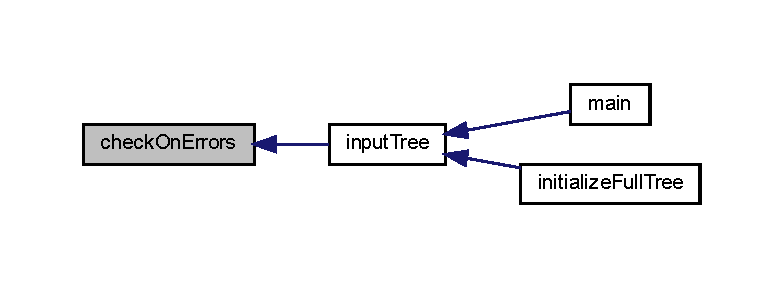
\includegraphics[width=350pt]{_open_brackets_header_8h_aaa006feb21d50122375e88727edfcfc7_icgraph}
\end{center}
\end{figure}
\mbox{\Hypertarget{_open_brackets_header_8h_ac803718224902c30b47da22d1d0e3cd6}\label{_open_brackets_header_8h_ac803718224902c30b47da22d1d0e3cd6}} 
\index{Open\+Brackets\+Header.\+h@{Open\+Brackets\+Header.\+h}!copy\+Vertex@{copy\+Vertex}}
\index{copy\+Vertex@{copy\+Vertex}!Open\+Brackets\+Header.\+h@{Open\+Brackets\+Header.\+h}}
\subsubsection{\texorpdfstring{copy\+Vertex()}{copyVertex()}}
{\footnotesize\ttfamily int copy\+Vertex (\begin{DoxyParamCaption}\item[{vector$<$ \mbox{\hyperlink{struct_node}{Node}} $>$ \&}]{tree,  }\item[{int}]{current\+Node }\end{DoxyParamCaption})}



Скопировать заданную вершину в векторе вершин 


\begin{DoxyParams}[1]{Аргументы}
\mbox{\tt in}  & {\em current\+Node} & индекс копируемой вершины \\
\hline
\mbox{\tt out}  & {\em tree} & вектор вершин \\
\hline
\end{DoxyParams}
\begin{DoxyReturn}{Возвращает}
индекс позиции скопированной вершины 
\end{DoxyReturn}
Граф вызовов\+:\nopagebreak
\begin{figure}[H]
\begin{center}
\leavevmode
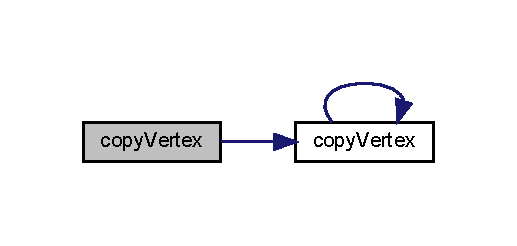
\includegraphics[width=248pt]{_open_brackets_header_8h_ac803718224902c30b47da22d1d0e3cd6_cgraph}
\end{center}
\end{figure}
Граф вызова функции\+:\nopagebreak
\begin{figure}[H]
\begin{center}
\leavevmode
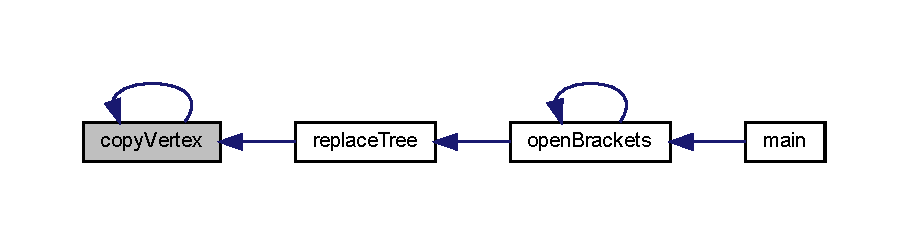
\includegraphics[width=350pt]{_open_brackets_header_8h_ac803718224902c30b47da22d1d0e3cd6_icgraph}
\end{center}
\end{figure}
\mbox{\Hypertarget{_open_brackets_header_8h_a0883c51a71859d6cb3eb32602e260e4c}\label{_open_brackets_header_8h_a0883c51a71859d6cb3eb32602e260e4c}} 
\index{Open\+Brackets\+Header.\+h@{Open\+Brackets\+Header.\+h}!crash\+Output@{crash\+Output}}
\index{crash\+Output@{crash\+Output}!Open\+Brackets\+Header.\+h@{Open\+Brackets\+Header.\+h}}
\subsubsection{\texorpdfstring{crash\+Output()}{crashOutput()}}
{\footnotesize\ttfamily bool crash\+Output (\begin{DoxyParamCaption}\item[{\mbox{\hyperlink{_open_brackets_header_8h_ab0df38968e4f03a3f1f6d6df0f31f45a}{Error\+Type}}}]{error }\end{DoxyParamCaption})}



Вывести сообщение об ошибке 


\begin{DoxyParams}[1]{Аргументы}
\mbox{\tt in}  & {\em error} & -\/ тип ошибки \\
\hline
\end{DoxyParams}
\begin{DoxyReturn}{Возвращает}
true при успешном выводе, false -\/ иначе 
\end{DoxyReturn}
Граф вызова функции\+:\nopagebreak
\begin{figure}[H]
\begin{center}
\leavevmode
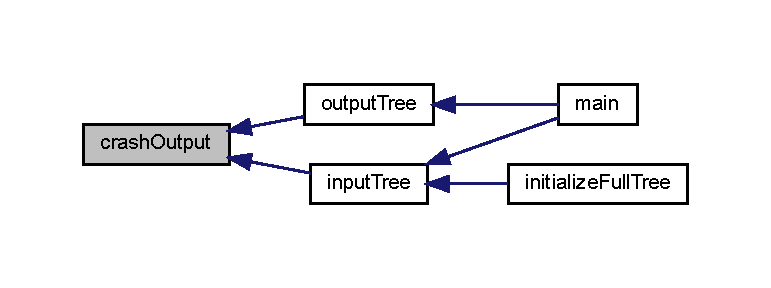
\includegraphics[width=350pt]{_open_brackets_header_8h_a0883c51a71859d6cb3eb32602e260e4c_icgraph}
\end{center}
\end{figure}
\mbox{\Hypertarget{_open_brackets_header_8h_ab583cc72190d7b0bc131d182dc947046}\label{_open_brackets_header_8h_ab583cc72190d7b0bc131d182dc947046}} 
\index{Open\+Brackets\+Header.\+h@{Open\+Brackets\+Header.\+h}!dfs\+Output@{dfs\+Output}}
\index{dfs\+Output@{dfs\+Output}!Open\+Brackets\+Header.\+h@{Open\+Brackets\+Header.\+h}}
\subsubsection{\texorpdfstring{dfs\+Output()}{dfsOutput()}}
{\footnotesize\ttfamily void dfs\+Output (\begin{DoxyParamCaption}\item[{ofstream \&}]{fout,  }\item[{vector$<$ \mbox{\hyperlink{struct_node}{Node}} $>$ \&}]{tree,  }\item[{int}]{current }\end{DoxyParamCaption})}



Вывести вершины дерева обходом в глубину 


\begin{DoxyParams}[1]{Аргументы}
\mbox{\tt in}  & {\em tree} & -\/ дерево разбора выражений \\
\hline
\mbox{\tt in}  & {\em current} & -\/ идентификатор вершины с которой производить вывод \\
\hline
\mbox{\tt out}  & {\em fout} & -\/ выходной поток \\
\hline
\end{DoxyParams}
Граф вызовов\+:\nopagebreak
\begin{figure}[H]
\begin{center}
\leavevmode
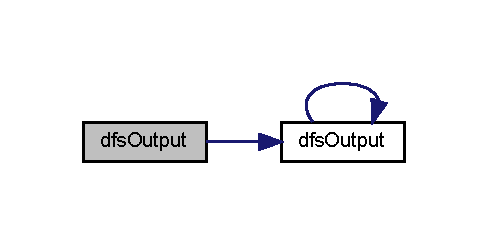
\includegraphics[width=234pt]{_open_brackets_header_8h_ab583cc72190d7b0bc131d182dc947046_cgraph}
\end{center}
\end{figure}
Граф вызова функции\+:\nopagebreak
\begin{figure}[H]
\begin{center}
\leavevmode
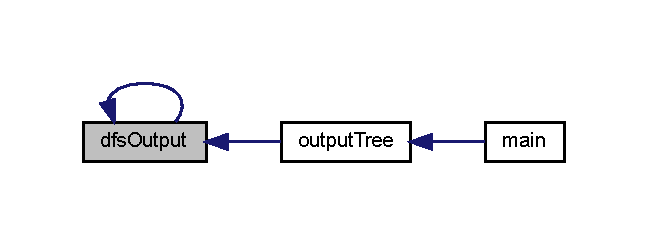
\includegraphics[width=311pt]{_open_brackets_header_8h_ab583cc72190d7b0bc131d182dc947046_icgraph}
\end{center}
\end{figure}
\mbox{\Hypertarget{_open_brackets_header_8h_a8e16eb9ea25217a287d10721c6d63e49}\label{_open_brackets_header_8h_a8e16eb9ea25217a287d10721c6d63e49}} 
\index{Open\+Brackets\+Header.\+h@{Open\+Brackets\+Header.\+h}!initialize\+Full\+Tree@{initialize\+Full\+Tree}}
\index{initialize\+Full\+Tree@{initialize\+Full\+Tree}!Open\+Brackets\+Header.\+h@{Open\+Brackets\+Header.\+h}}
\subsubsection{\texorpdfstring{initialize\+Full\+Tree()}{initializeFullTree()}}
{\footnotesize\ttfamily void initialize\+Full\+Tree (\begin{DoxyParamCaption}\item[{vector$<$ \mbox{\hyperlink{struct_node}{Node}} $>$ \&}]{input\+Tree }\end{DoxyParamCaption})}



Заполнить входное дерево до максимального размера 


\begin{DoxyParams}[1]{Аргументы}
\mbox{\tt out}  & {\em input\+Tree} & -\/ дерево разбора выражений \\
\hline
\end{DoxyParams}
Граф вызовов\+:\nopagebreak
\begin{figure}[H]
\begin{center}
\leavevmode
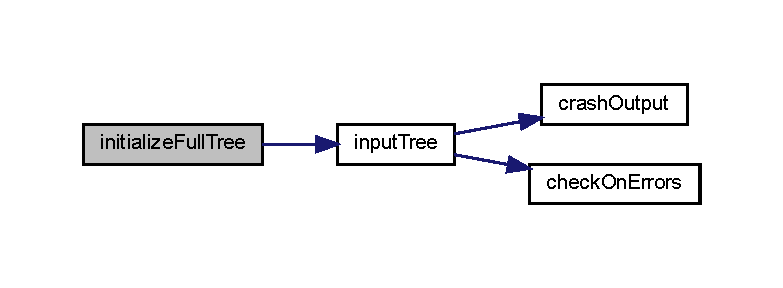
\includegraphics[width=350pt]{_open_brackets_header_8h_a8e16eb9ea25217a287d10721c6d63e49_cgraph}
\end{center}
\end{figure}
\mbox{\Hypertarget{_open_brackets_header_8h_a797b21a870af459209e0b303375490e6}\label{_open_brackets_header_8h_a797b21a870af459209e0b303375490e6}} 
\index{Open\+Brackets\+Header.\+h@{Open\+Brackets\+Header.\+h}!input\+Tree@{input\+Tree}}
\index{input\+Tree@{input\+Tree}!Open\+Brackets\+Header.\+h@{Open\+Brackets\+Header.\+h}}
\subsubsection{\texorpdfstring{input\+Tree()}{inputTree()}}
{\footnotesize\ttfamily bool input\+Tree (\begin{DoxyParamCaption}\item[{int}]{argc,  }\item[{char $\ast$}]{argv\mbox{[}$\,$\mbox{]},  }\item[{ifstream \&}]{fin,  }\item[{vector$<$ \mbox{\hyperlink{struct_node}{Node}} $>$ \&}]{tree,  }\item[{int \&}]{root }\end{DoxyParamCaption})}



Ввести заданное дерево разбора выражений 


\begin{DoxyParams}[1]{Аргументы}
\mbox{\tt in}  & {\em argc} & -\/ аргумент командной строки \\
\hline
\mbox{\tt in}  & {\em argv\mbox{[}$\,$\mbox{]}} & -\/ аргументы командной строки \\
\hline
\mbox{\tt in}  & {\em fin} & -\/ входной поток \\
\hline
\mbox{\tt out}  & {\em tree} & -\/ дерево разбора выражений \\
\hline
\mbox{\tt out}  & {\em root} & -\/ индекс корня дерева разбора выражений \\
\hline
\end{DoxyParams}
\begin{DoxyReturn}{Возвращает}
true -\/ при успешном ввводе, false -\/ иначе 
\end{DoxyReturn}

\begin{DoxyExceptions}{Исключения}
{\em U\+N\+K\+N\+O\+W\+N\+\_\+\+F\+I\+L\+E\+\_\+\+E\+X\+T\+E\+N\+S\+I\+ON} & -\/ неверно указано расширение входного файла \\
\hline
{\em I\+N\+P\+U\+T\+\_\+\+F\+I\+L\+E\+\_\+\+N\+O\+T\+\_\+\+E\+X\+I\+ST} & -\/ не существует или не найден входной файл \\
\hline
{\em W\+R\+O\+N\+G\+\_\+\+D\+A\+T\+A\+\_\+\+F\+O\+R\+M\+AT} & -\/ неверный формат данных во входном файле \\
\hline
{\em T\+R\+E\+E\+\_\+\+S\+I\+Z\+E\+\_\+\+O\+U\+T\+\_\+\+O\+F\+\_\+\+R\+A\+N\+GE} & -\/ размер дерева во входном файле вне поддерживаемого диапазона \\
\hline
\end{DoxyExceptions}
Граф вызовов\+:\nopagebreak
\begin{figure}[H]
\begin{center}
\leavevmode
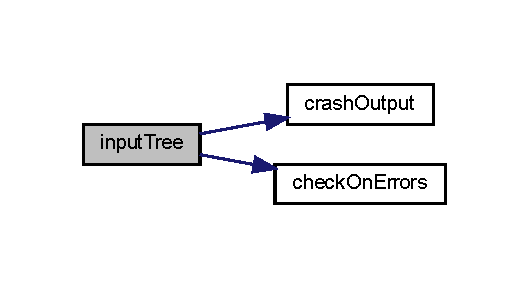
\includegraphics[width=254pt]{_open_brackets_header_8h_a797b21a870af459209e0b303375490e6_cgraph}
\end{center}
\end{figure}
Граф вызова функции\+:\nopagebreak
\begin{figure}[H]
\begin{center}
\leavevmode
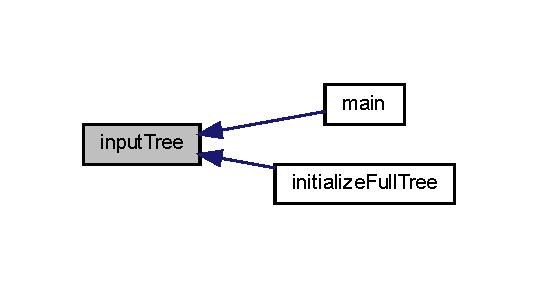
\includegraphics[width=258pt]{_open_brackets_header_8h_a797b21a870af459209e0b303375490e6_icgraph}
\end{center}
\end{figure}
\mbox{\Hypertarget{_open_brackets_header_8h_a25881c5367e2db6534a50cd6b17ed6a1}\label{_open_brackets_header_8h_a25881c5367e2db6534a50cd6b17ed6a1}} 
\index{Open\+Brackets\+Header.\+h@{Open\+Brackets\+Header.\+h}!is\+Equal\+Trees@{is\+Equal\+Trees}}
\index{is\+Equal\+Trees@{is\+Equal\+Trees}!Open\+Brackets\+Header.\+h@{Open\+Brackets\+Header.\+h}}
\subsubsection{\texorpdfstring{is\+Equal\+Trees()}{isEqualTrees()}}
{\footnotesize\ttfamily bool is\+Equal\+Trees (\begin{DoxyParamCaption}\item[{vector$<$ \mbox{\hyperlink{struct_node}{Node}} $>$}]{first\+Tree,  }\item[{int}]{root\+Of\+First\+Tree,  }\item[{vector$<$ \mbox{\hyperlink{struct_node}{Node}} $>$}]{second\+Tree,  }\item[{int}]{root\+Of\+Second\+Tree }\end{DoxyParamCaption})}



Сравнить два дерева между собой 


\begin{DoxyParams}[1]{Аргументы}
\mbox{\tt in}  & {\em first\+Tree} & -\/ первое дерево \\
\hline
\mbox{\tt in}  & {\em root\+Of\+First\+Tree} & -\/ индекс корневого узла первого дерева \\
\hline
\mbox{\tt in}  & {\em second\+Tree} & -\/ второе дерево \\
\hline
\mbox{\tt in}  & {\em root\+Of\+Second\+Tree} & -\/ индекс корневого узла второго дерева \\
\hline
\end{DoxyParams}
\begin{DoxyReturn}{Возвращает}
true -\/ если деревья совпадают, false -\/ если деревья разные 
\end{DoxyReturn}
Граф вызовов\+:\nopagebreak
\begin{figure}[H]
\begin{center}
\leavevmode
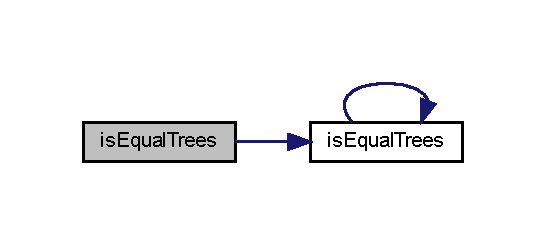
\includegraphics[width=262pt]{_open_brackets_header_8h_a25881c5367e2db6534a50cd6b17ed6a1_cgraph}
\end{center}
\end{figure}
Граф вызова функции\+:\nopagebreak
\begin{figure}[H]
\begin{center}
\leavevmode
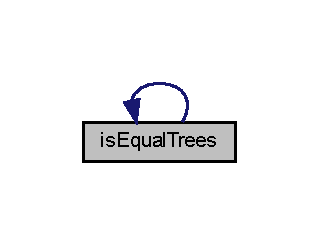
\includegraphics[width=153pt]{_open_brackets_header_8h_a25881c5367e2db6534a50cd6b17ed6a1_icgraph}
\end{center}
\end{figure}
\mbox{\Hypertarget{_open_brackets_header_8h_a18dcaf2e91cb700bc12aae6fd594f0e8}\label{_open_brackets_header_8h_a18dcaf2e91cb700bc12aae6fd594f0e8}} 
\index{Open\+Brackets\+Header.\+h@{Open\+Brackets\+Header.\+h}!open\+Brackets@{open\+Brackets}}
\index{open\+Brackets@{open\+Brackets}!Open\+Brackets\+Header.\+h@{Open\+Brackets\+Header.\+h}}
\subsubsection{\texorpdfstring{open\+Brackets()}{openBrackets()}}
{\footnotesize\ttfamily void open\+Brackets (\begin{DoxyParamCaption}\item[{vector$<$ \mbox{\hyperlink{struct_node}{Node}} $>$ \&}]{tree,  }\item[{int}]{current\+Node }\end{DoxyParamCaption})}



Раскрыть скобки в заданном выражении 


\begin{DoxyParams}[1]{Аргументы}
\mbox{\tt in}  & {\em current\+Node} & -\/ индекс узла дерева с которого следует раскрывать скобки \\
\hline
\mbox{\tt out}  & {\em tree} & -\/ дерево разбора выражений \\
\hline
\end{DoxyParams}
Граф вызовов\+:\nopagebreak
\begin{figure}[H]
\begin{center}
\leavevmode
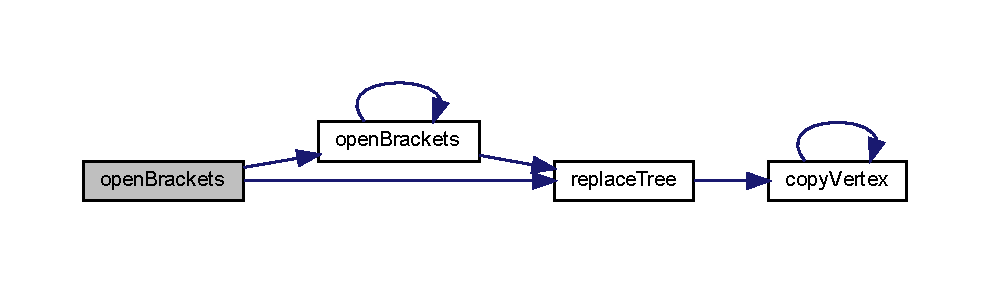
\includegraphics[width=350pt]{_open_brackets_header_8h_a18dcaf2e91cb700bc12aae6fd594f0e8_cgraph}
\end{center}
\end{figure}
Граф вызова функции\+:\nopagebreak
\begin{figure}[H]
\begin{center}
\leavevmode
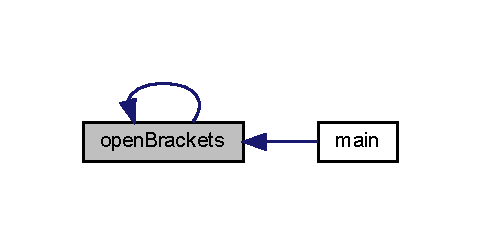
\includegraphics[width=231pt]{_open_brackets_header_8h_a18dcaf2e91cb700bc12aae6fd594f0e8_icgraph}
\end{center}
\end{figure}
\mbox{\Hypertarget{_open_brackets_header_8h_a7eb4dce1633fdd03c97d7fd46f02089f}\label{_open_brackets_header_8h_a7eb4dce1633fdd03c97d7fd46f02089f}} 
\index{Open\+Brackets\+Header.\+h@{Open\+Brackets\+Header.\+h}!output\+Tree@{output\+Tree}}
\index{output\+Tree@{output\+Tree}!Open\+Brackets\+Header.\+h@{Open\+Brackets\+Header.\+h}}
\subsubsection{\texorpdfstring{output\+Tree()}{outputTree()}}
{\footnotesize\ttfamily bool output\+Tree (\begin{DoxyParamCaption}\item[{int}]{argc,  }\item[{char $\ast$}]{argv\mbox{[}$\,$\mbox{]},  }\item[{ofstream \&}]{fout,  }\item[{vector$<$ \mbox{\hyperlink{struct_node}{Node}} $>$ \&}]{tree,  }\item[{int \&}]{current }\end{DoxyParamCaption})}



Вывести дерево разбора выражений 


\begin{DoxyParams}[1]{Аргументы}
\mbox{\tt in}  & {\em argc} & -\/ аргумент командной строки \\
\hline
\mbox{\tt in}  & {\em argv\mbox{[}$\,$\mbox{]}} & -\/ аргументы командной строки \\
\hline
\mbox{\tt in}  & {\em tree} & -\/ дерево разбора выражений \\
\hline
\mbox{\tt in}  & {\em current} & -\/ индекс вершины, с которой производить вывод дерева \\
\hline
\mbox{\tt out}  & {\em fout} & -\/ выходной поток \\
\hline
\end{DoxyParams}
\begin{DoxyReturn}{Возвращает}
true -\/ при успешном выводе, false -\/ иначе 
\end{DoxyReturn}

\begin{DoxyExceptions}{Исключения}
{\em U\+N\+K\+N\+O\+W\+N\+\_\+\+F\+I\+L\+E\+\_\+\+E\+X\+T\+E\+N\+S\+I\+ON} & -\/ неверно указано расширение выходного файла \\
\hline
{\em O\+U\+T\+P\+U\+T\+\_\+\+F\+I\+L\+E\+\_\+\+C\+R\+E\+A\+T\+I\+O\+N\+\_\+\+F\+A\+I\+L\+ED} & -\/ невозможно создать выходной файл \\
\hline
\end{DoxyExceptions}
Граф вызовов\+:\nopagebreak
\begin{figure}[H]
\begin{center}
\leavevmode
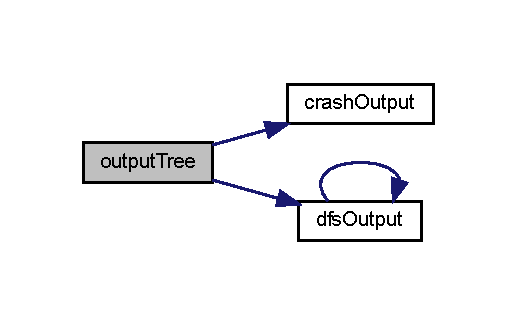
\includegraphics[width=248pt]{_open_brackets_header_8h_a7eb4dce1633fdd03c97d7fd46f02089f_cgraph}
\end{center}
\end{figure}
Граф вызова функции\+:\nopagebreak
\begin{figure}[H]
\begin{center}
\leavevmode
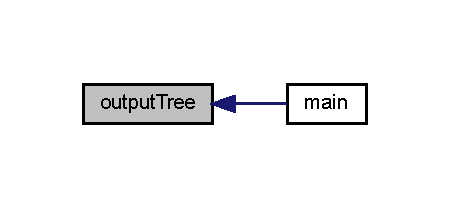
\includegraphics[width=216pt]{_open_brackets_header_8h_a7eb4dce1633fdd03c97d7fd46f02089f_icgraph}
\end{center}
\end{figure}
\mbox{\Hypertarget{_open_brackets_header_8h_a61492c3970be2433213dcd7344c27426}\label{_open_brackets_header_8h_a61492c3970be2433213dcd7344c27426}} 
\index{Open\+Brackets\+Header.\+h@{Open\+Brackets\+Header.\+h}!replace\+Tree@{replace\+Tree}}
\index{replace\+Tree@{replace\+Tree}!Open\+Brackets\+Header.\+h@{Open\+Brackets\+Header.\+h}}
\subsubsection{\texorpdfstring{replace\+Tree()}{replaceTree()}}
{\footnotesize\ttfamily void replace\+Tree (\begin{DoxyParamCaption}\item[{vector$<$ \mbox{\hyperlink{struct_node}{Node}} $>$ \&}]{tree,  }\item[{int}]{current\+Node,  }\item[{string}]{operation }\end{DoxyParamCaption})}



Перестроить часть дерева ниже текущего узла в соответствии с операцией 


\begin{DoxyParams}[1]{Аргументы}
\mbox{\tt in}  & {\em current\+Node} & -\/ индекс узла дерева с которого следует перестраивать дерево \\
\hline
\mbox{\tt in}  & {\em operation} & -\/ операция текущего узла \\
\hline
\mbox{\tt out}  & {\em tree} & -\/ дерево разбора выражений \\
\hline
\end{DoxyParams}
Граф вызовов\+:\nopagebreak
\begin{figure}[H]
\begin{center}
\leavevmode
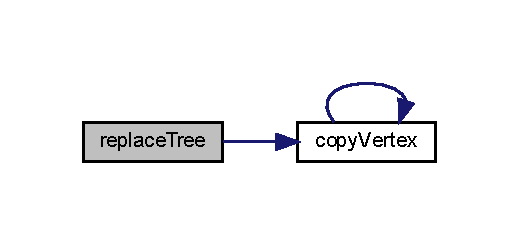
\includegraphics[width=249pt]{_open_brackets_header_8h_a61492c3970be2433213dcd7344c27426_cgraph}
\end{center}
\end{figure}
Граф вызова функции\+:\nopagebreak
\begin{figure}[H]
\begin{center}
\leavevmode
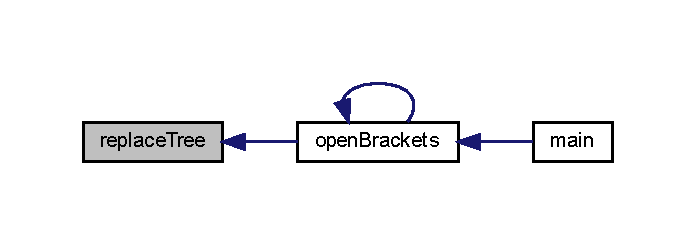
\includegraphics[width=334pt]{_open_brackets_header_8h_a61492c3970be2433213dcd7344c27426_icgraph}
\end{center}
\end{figure}

%--- End generated contents ---

% Index
\backmatter
\newpage
\phantomsection
\clearemptydoublepage
\addcontentsline{toc}{chapter}{Алфавитный указатель}
\printindex

\end{document}
